%%% renderer.tex

\documentclass[UTF8,8pt]{report}
% 目录
\usepackage[titles]{tocloft}
% 引入中文
\usepackage{ctex} 
% 超链接
\usepackage[colorlinks,linkcolor=blue]{hyperref}
\usepackage{url}
% 引用
\usepackage{cite}
%\usepackage{natbib}
% 图片
\usepackage{graphicx}
% 数学
% 矩阵
\usepackage{mathtools}
\usepackage{amssymb}
\usepackage{amsmath}
\usepackage{arydshln}
% 给方程,图片,表格编号,section可能换成chapter
\renewcommand{\theequation}{\arabic{section}-\arabic{equation}}
\renewcommand{\thefigure}{\arabic{section}-\arabic{figure}}
\renewcommand{\thetable}{\arabic{section}-\arabic{table}}
% 嵌入代码
\usepackage{listings}

\setlength{\baselineskip}{1.5em} % 行间距
\setlength{\parskip}{1.0ex} % 段间距
\setlength{\parindent}{0pt} % 段落缩进

% 文档开始
\begin{document}
%-----使用封面代替
%\title{renderer-title}
%\maketitle
%-----封面
\begin{center}
    \quad \\
    \vspace{3cm}
    \hspace{1cm}\Huge{Renderer渲染器} \\
    \small{关于渲染器知识的整理} \\
    \vspace{1cm}
    \hspace{1cm}\Large{李美杰} \\
    \vspace{0.5cm}
    \hspace{1cm}\Large{2019.9.13}
    \clearpage
\end{center}
%-----

%-----留白
\thispagestyle{empty}
\clearpage
%-----

%-----目录
\tableofcontents
\clearpage
%-----

% 代码区域样式
\lstset{
    language=C,
    numbers=left,
    frame=box
}

%-----正文
\chapter{Renderering}

在渲染方面上的研究与优化已经发展成熟,已成为一个非常复杂的系统了,本文的目标是从理解渲染的技术原理,从软渲染,到CPU,再到GPU。
为简化,我们以图元三角形为例,主要有两个阶段:
\begin{itemize}
    \item {决定那些像素坐标构成这个三角形}
    \item {决定这些像素的颜色值是多少,这个过程就是着色shading}
\end{itemize}
它们分别对应着图形学中另外两个概念,光栅化和光照模型。

\section{Rasterize}
光栅化
图形学中,是物理的三维世界,如何把三维物体在二维屏幕上显示,需要把它的三维属性都降为二维的结果,大致存在以下几个步骤:

\begin{itemize}
    \item {坐标变换}
    \item {属性计算,如颜色,纹理,alpha等}
    \item {光栅化}
\end{itemize}

\textsf{目前大众屏幕分辨率为1920x1080,在二维屏幕渲染时,内存中的FrameBuffer只保存着1920x1080个屏幕点的颜色,然后再映射到屏幕上面。
光栅化的,就是计算出1920x1080个点的颜色值的过程。把物体的数学描述转换为屏幕的像素值,是从连续到离散,即物理的坐标是浮点数,而屏幕坐标是整数,光栅化的过程是一个近似的过程。
在一些图形处理软件中就是把矢量图形转化成像素点的过程。}

\begin{description}
    \item [主动:] \textsf{定时渲染,与时间关系比较严格的}
    \item [被动:] \textsf{请求渲染,与动画相关的,以流畅为结果}
\end{description}

\text{目前处理光照生成图像的过程中,计算的级别有:}

\begin{itemize}
    \item {逐顶点光照,在每个顶点计算光照,在渲染图元内部进行插值,光照模型中的非线性关系会产生问题}
    \item {逐像素光照,Phong着色,在fragment对顶点法线进行插值}
\end{itemize}


\section{Photorealistic Rendering}

真实感图形技术包括消隐技术,光照模型,明暗处理和纹理,阴影生成等

\begin{itemize}
    \item {局部光照,仅处理光源直接照射物体表面的光照模型,与光栅化渲染算法相适应的,一次只考虑
    一个像素的光照强度,逐像素的光照计算,不能得到其他像素的光照影响值}
    \begin{itemize}
        \item {Lambert漫反射模型,不能很好处理镜面与高光}
        \item {Gourand}
        \item {Phong,支持高光与镜面}
        \item {Blinn-Phong,速度快,目前商业普遍使用}
        \item {Cook-Torrance,以双向反射的基础上}
    \end{itemize}
    \item {全局光照,基于光学物理原理,光照强度的计算依赖于光能在现实世界中的传播,考虑光线与整个场景中
    各物体表面以及物体表面之间的相互影响,包括多次反射、透射、散射等,成熟应用在离线渲染中}
    \begin{itemize}
        \item {光线跟踪,模拟光从光源出发经过若干次反射、折射达到摄像机的过程,由于只有最终到达摄像机的光线
        才对生成图像有贡献,实现中是以摄像机逆向发出光线,以寻求达到光源的路径。}
        \begin{itemize}
            \item {路径跟踪Path Tracing}
            \item {递归光线追踪Whitte-type}
            \item {分布式光线追踪Distrubution}
            \item {双向路径追踪Bidirectional Path}
            \item {Metropolis}
        \end{itemize}
        \item {辐射度算法,是一种物体空间的算法,用于解离散点或环境中表面曲面面片的光强度问题,而不是解图像平面
        投影的像素问题}
        \item {光子映射,改善漫反射辉映,焦散等全局光照效果,还无法应用在实时渲染中}
    \end{itemize}
\end{itemize}

\section{Non-Photorealistic Rendering}
对于某些场景,不需要真实感,需要一些艺术化的表现
钢笔素描的生成,
中国国画与书法的生成。
\newline
\textbf{Artistic Shading},艺术渲染,模拟人简画的素描之类的,是一种根据轮廓来来抽象效果。

\section{Image-Based Rendering}

IBR,基于图像的渲染,完全摒弃传统的先建模,然后确定光源的渲染方法,
它直接从一系列已知的图像中生成新颖的视口图像,适用于野外极其复杂场景的生成和漫游。

\section{Stereo Rendering}
立体渲染,是一种让人眼能够感受到立体效果的渲染方式,需要两个camera对同一个场景进行渲染,两个view得到
的图像略有差异(两个camera的投影矩阵的差异),让人产生深度的视觉效果。一般分左右两个camera。

通常渲染完成后,整张图像还需要一次后处理Barrel distortion桶形失真,以抵消VR设备固有的pincushion distortion枕形失真。
\begin{figure}[h]
    \centering
    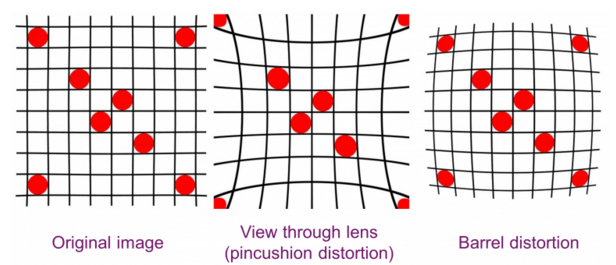
\includegraphics[width=\textwidth]{images/Optimising-OpenGL-ES-for-mobile-VR-lens-distortion.png}
    \caption{Phong Shading Model}
\end{figure}


\section{Deferred Shading}

\begin{itemize}    
    \item {不能使用混合技术}
    \item {占用较高的显存}
    \item {光照的开销与场景复杂度无关}
    \item {Shader可以访问深度和其他像素信息}
    \item {每个像素对每个光源仅运行一次,被遮挡的像素是不会参与计算}
    \item {材质与光照的Shader是分开的}
\end{itemize}

\section{Anti-Aliasing}

渲染中,最终结果是一张图像,其最小单位就是像素。像素是很小的一个色块,当图像分辨率足够高时,色块足够小,
相邻色块之间的颜色差异人眼是很难辨别的,看到的就是一副细腻顺滑的图像,当分辨率较低时,为了填充同样大小的
屏幕,色块的尺寸就相应变大了,色块之间的差异就很难被忽视了。因为屏幕是点阵显示,就造成物理上无法避免的问题。

\subsection{Samping}

锯齿产生的主要情况有:
\begin{itemize}
    \item {几何走样,几何物体的边缘有锯齿,对几何边缘采样不足导致的}
    \item {着色走样,渲染方程中的着色公式采样不足导致的,就是高光闪烁就是一种情况}
    \item {时间走样,对高速物体的采样不足,比如播放的动画发生跳变}
\end{itemize}

按照香农采样定律的理论,要想通过对采样后的信号进行重建Reconstruct来获得原始信号,就必须保证采样频率不低于
原始信号最高频率的两倍。

\begin{figure}[h]
    \centering
    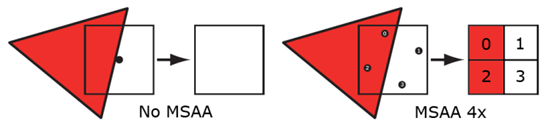
\includegraphics[width=\textwidth]{images/ssaa.png}
    \caption{SuperSampling AA}
\end{figure}

图元覆盖在色块上,简单的判断就是是否中心点被覆盖否,但是这样判断会引入图元的位置差异结果,将色块进一步细分成不同的
小块,对每个小块进行判断,再由这些小块的颜色加权计算出来,这就是通过采样来得到更好的颜色值。

带来的问题就是一次pass对Pixel/Fragment shader需要4倍的像素处理,另一种思路就是多次pass的Accumulation Buffer方法,
每次pass时都进行一定程度的偏移(通常0.5个像素),最后进行累积后再平均,但是多次绘制需要进行Buffer之间的
数据拷贝,消耗也是非常大的。


\subsection{Sampling Pattern}

先说说采样点纹,即才采样点在像素色块中的分布方式。研究表明人眼感官影响最严重的锯齿现象是由水平或垂直边缘导致的,其次是45度夹角的边缘。
Rotated Grid SuperSampling就是把采样点旋转45度的来提升AA的质量。

\subsection{MSAA}

Multisampling Antialiasing是改进版,SSAA对每次FS需要四次sample计算,假设色块任意点颜色值近似相同,把sample后的值存入
对应的buffer中,利用这些覆盖点的sample点进行插值,就是Centroid Sampling(Interplotation),这个动作通常由硬件自动完成。

MSAA渲染完成后,需要将subsample的数据转换为pixel color,这个过程称为MSAA 解析Resolve。现代GPU的FS或Compute Shader都可以直接
操作MSAA的处理过程,可以使用不同的filter来实现图像的AA重建,可以参考\cite{OpenGLMultiSampling}

下图来自Direct3D11的Graphics Pipeline\cite{RasterizationRules} 

\begin{figure}[h]
    \centering
    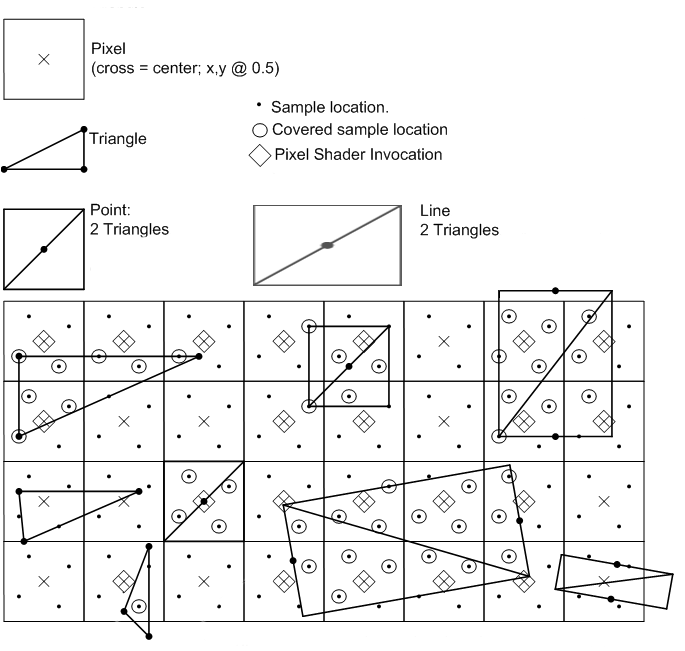
\includegraphics[width=\textwidth]{images/d3d10-rasterrulesmsaa.png}
    \caption{MSAA sample 4 for d3d10}
\end{figure}

\subsection{TAA}

上面讨论的都是在同一帧中,像素在不同位置上的采样处理,可认为是空间上的方法。现在从时间角度上来分析,实时渲染在一秒内会进行
多帧的连续渲染,前后两帧的重复度极高,利用之前多帧的渲染结果提取信息来优化渲染结果是否可行呢?这就是Temporal AA。 

使用TAA好处是同一帧没有额外的采样消耗,只需要对多帧结果进行一个融合即可,但多帧的重叠度与加权值的处理不够好时,会出现抖动闪烁
的瑕疵。解决方法有两种,一是只对低速物体使用TAA,一是对当前帧与之前帧的画面进行映射与投影校正reprojection,常见的使用速度
贴图velocity buffer。TAA+Velocity Buffer与Deferred Rendering是不兼容的。

\subsection{MLAA}

锯齿产生在于几何形状与颜色交界处,如果能事先得到这些信息,就可以针对性的进行抗锯齿处理,2019年Reshetov提出一种沿着边界线
edge进行的AA方法,称为Morphological Antialiasing, 此方法侧重于边界线的定位与重构。



\chapter{Illumination Model}

当光照射到物体表面时,物体会对光发生反射、透射、吸收、衍射、折射、干涉等。其中被物体吸收的部分转化为热。
反射、透射的光会进入人的视觉系统,使我们看见物体。为了模拟仿真这一真实的现象,建立一些数学模型来替代复杂的真实
物理模型,这些模型就称为光照模型。

\section{Lamertian}
1970年Bouknight提出了第一个光反射模型。1971Gourand提出“漫反射模型+插值”的思想,称为Gourand明暗处理。
即出物体表面朝向(即法线)是确定物体表面上一点光强的主要因素,用Lambert漫反射定律计算物体表面上各多
边形的光强,对光照射不到的使用环境光代替。
\textbf{Lambert's cosin law},告诉我们曲面表面的颜色c与表面法线和光源方向的夹角的余弦值cosine成正比。

\begin{align*}
c \propto cos(\theta) \\
c \propto n \cdot l 
\end{align*}

漫反射:当光线从光源照射到曲面表面时,表面向每个方向散射辐射量。漫反射符合兰伯特定律。

\begin{align*}    
c_{diffuse} = max(0, \hat{n} * \hat{l}), \\
c_{ambient} = Kd * Ia, \\
c_{light} = Kd * Il, \\ 
c_{final} = c_{ambient} + c_{light}c_{diffuse}, \\
0 < Kd < 1, 
\end{align*}

Kd是材质对环境光的反射系数,Ia表示环境光强度,Il表示点光源强度
注意,这里存在一个前提,就是假设光源方向l不依赖渲染物体的位置信息,就是光与渲染对象有足够的远,就是
方向光directional light。

\section{Phong Model}

Phong模型引入镜面光,即ADS(ambient,diffuse,specular),认为镜面与反射的光强和反射光线与视线的夹角相关

\begin{figure}[htbp]
    \centering
    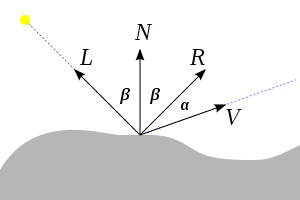
\includegraphics[width=0.8\textwidth]{images/phong-shading-model.png}
    \caption{Phong-Model-Specular}\label{Phong-Model-Specular}
\end{figure}

图\ref{Phong-Model-Specular}中的$\alpha$ 很小时,就是高光效果

\begin{align*}
    R = -L + 2(L \cdot N) * N \\
    I_{spec}=Ks * Il * (dot(V, R))^N_{s}
\end{align*}

Ks为镜面反射系数,Ns为高光指数。

\begin{figure}[htbp]
    \centering
    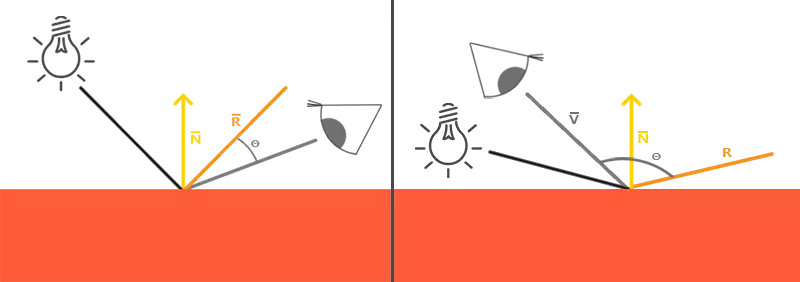
\includegraphics[width=0.8\textwidth]{images/classical-phong.png}
    \caption{Phong-Problem}\label{Phong-Problem}
\end{figure}
图\ref{Phong-Problem}模型中存在一个问题就是$\alpha$的角度大于90度时,会导致结果为负,产生假象。

Blinn-Phong是基于Phong的修正模型,

\begin{figure}[htbp]
    \centering
    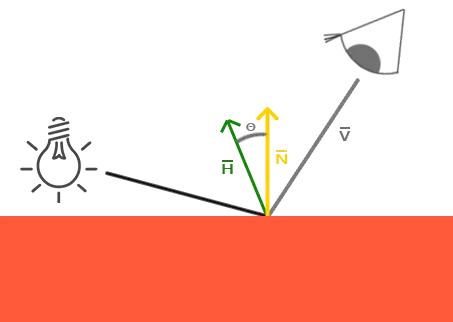
\includegraphics[width=0.8\textwidth]{images/blinn-phong.png}
    \caption{Blinn-Phong}\label{Blinn-Phong}
\end{figure}

图\ref{Blinn-Phong}通过半角来方法来解决可能出现角度大于90度的问题。

\begin{align*}
    H = \frac{L + V}{|L + V|}, \\
    I_{spec} = Ks * Il * (dot(N, H))^N_{s}
\end{align*}

H是入射光线方向L与视线方向V的中间向量,称之为半角向量。Classical-Phong更真实,Blinn-Phong高光更柔和,且计算速度较快,
实际中应用更广,OpenGL和DirectX渲染管线中是默认渲染模型。

\section{Global Illumination}
现实中的物体表面会接收大部分或全部来自其他反射出来的光线,称为indirect lighting或mutual illumination。
局部光照模型只考虑光对物体的照明,忽略了物体间的相互影响,其一般公式可以表示为

\begin{align*}
    I = I_{abmient} + \sum_{i}^{N}I_{light}\frac{1}{k_{c}+k_{l} \cdot d_{i} + k_{q} \cdot d_{i}^2}
    \left[ k_{d}(N \cdot L) + k_{s}(R \cdot V)^n \right]
\end{align*}

每个光源对物体的影响主要包括漫反射和镜面反射两部分,局部照明的阴影算法需要单独考虑。
\newline
全局照明考虑更全面,它自带阴影效果。它主要有两种算法:
\begin{itemize}
    \item {光线追踪法, 关注于镜面反射光,可严格追踪反射光线的方向,实际中采用逆向追踪法,减少计算量}
    \item {辐射度法, 关注于漫反射光,}
\end{itemize}
基本模型是 
\newline

\begin{align*}
    I_r = I_{ia}R_{a} + \sum_{l}I_{il}(N \cdot L_{l})d \omega_{il}(sR_{s} + dR_{d})
\end{align*}

其中的环境光和漫反射分量不依赖于观察者的位置View's Position。假设表面是由微面元组成microfacet,其镜面分量为:
\newline

\begin{align*}
    R_s = \frac{F}{\pi} \frac{DG}{\pi (N \cdot L)(N \cdot V)}
\end{align*}

为更加丰富,引入了几何项G,Fresnel项F,粗糙度项D。
\newline

\textbf{粗糙度项D},代表了可以有效反射光的那一部分微面元所占的比例,有多种分别函数。
高斯分布模型
\newline

\begin{align*}
    D = ce^{-(\alpha / m)^2}
\end{align*}

Bechmann分布函数
\newline

\begin{align*}
    D = \frac{1}{m^2cos^4(\theta)}e^-(tan\alpha / m)^2
\end{align*}

\textbf{几何项G},几何衰减项,表现了微小面元之间的互相遮挡shadowing and masking所造成的影响。
\newline

\begin{align*}
    G = \left\{
        1, \frac{2(N \cdot H)(N \cdot V)}{(V \cdot H)}, \frac{2(N \cdot H)(N \cdot L)}{(V \cdot H)} 
    \right\}
\end{align*}

\textbf{Fresnel项F},描述了在每一个微面元上光是如何反射,与入射角和波长相关。
\newline

\begin{align*}
    c = cos(\theta) = V \cdot H \\
    g^2 = n^2 + c^2 - 1 \\
F = \frac{1(g-c)^2}{2(g+c)^2} \left\{ 1+\frac{[c(g+c)-1]^2}{[c(g-c)+1]^2} \right\}
\end{align*}

\section{Physically based Rendering}

PBR refers to the concept of using realistic shading/lighting models along with measured surface values to accurately represent real-world materials

\section{notes}

多边形渲染会降低渲染速度,而要丰富的表面就需要更多的细节,要模拟表面的凹凸感,
与其增加多边形,不如利用光照的明暗来表示凹凸感,骗过人眼。光照模型都跟光线向量和表面法向量的夹角有关。
扰动就是影响法线向量与光线向量的夹角发生变化,从而产生明暗的变化,给人凹凸感。这就是使用法线贴图在低模中获得高模的凹凸的表面光照效果

\chapter{Texture}

\begin{abstract}
    纹理是比直接用颜色值更具有连续性, 对每个光栅化的屏幕坐标(usually a pixel center), 
    算出它的uv坐标(利用三角形顶点重心坐标插值using barycentric coordinates), 
    用uv坐标去查询texture上的颜色值,把这个颜色值当作
    漫反射系数Kd使用albedo Kd(Blinn-Phong reflectance model)
    \begin{enumerate}
        \item \text{for each rasterized screen sample(x,y):}
        \begin{enumerate}
            \item \text{(u,v) = evaluate texture coordinate at (x,y)}
            \item \text{texcolor = texture.sample(u,v)}
            \item \text{set sample's color to texcolor}
        \end{enumerate}
    \end{enumerate}    
\end{abstract}

可阅读
Chapter 20 Textures and Texture Mapping\cite{CGPP3ed}

Chapter 11 Texture Mapping\cite{FCG4ed}

Chapter 6 Texturing\cite{RTR4ed}

\section{Texture Mapping}
纹理映射,即纹理坐标的生成函数,纹理空间之内任意一个二维坐标都在[0,1]之内。

\begin{figure}[h]
    \centering
    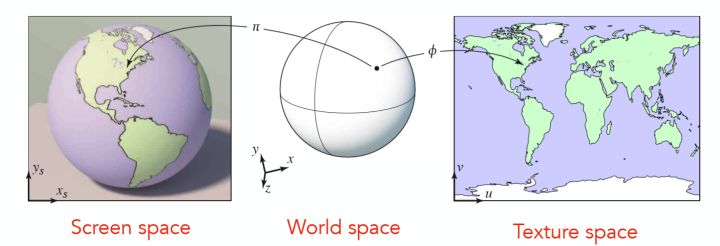
\includegraphics[width=1\textwidth]{images/texture-mapping-sphere.jpg}
    \caption{地球仪}    
\end{figure}

纹理应用在表面的大致逻辑是
\begin{lstlisting}
    Color texture_lookup(Texture t, float u, float v) {
        int i = round(u * t.width() - 0.5);
        int j = round(v * t.height() - 0.5);
        return t.get_pixel(i,j);
    }
    Color shade_surface_point(Surface s, Point p, Texture t) {
        Vector normal = s.get_normal(p);
        (u,v) = s.get_texcoord(p);
        Color diffuse_color = texture_lookup(t, u, v);
        // compute shading using diffuse_color and normal 
        // return shading result    
    }
\end{lstlisting}
就是对每个光栅化的屏幕坐标算出它的uv坐标(利用三角形顶点重心坐标插值),再利用uv坐标取查询texture
上的颜色,把这个颜色信息当作漫反射系数Kd。


以顶视图Y轴方向来看,对X(S)和Z(T)生成对应的纹理坐标值UV,即Y平面为UV展开

\begin{enumerate}
    \item \textsf{遍历所有点得到lowestX和highestX,lowestX=-12.00,highestX=134.56}
    \item \textsf{得到绝对范围 range=(lowest - highest) * -1 = (-12.00-134.56)*-1=146.56}
    \item \textsf{与0的偏移值offset=0-lowestX=0 - (-12.00)=12}
    \item \textsf{vertex x=87.45, absoluteX=X+offset=87.45+12=99.45}
    \item \textsf{get S value, s = absoluteX / range = 99.45/145.56=0.679}
    \item \textsf{do the same for Z axis to get T value}
\end{enumerate}

从Image Space到Texture space(T), 存在一个函数映射,从World space中Surface(S), 数学模型如下:

\begin{align*}
    \phi &: S \rightarrow T \\
    &: (x,y,z) \rightarrow (u,v)
\end{align*}

函数$\phi$存在很多种形式

\subsection{Basic Texturing}

是最基本的纹理映射,仿射粘贴(affine gluing),把图像粘贴到一个三角形,通过三角形的三个顶点指定纹理坐标方式,
顶点存储uv值,并在特定的texture中获取相应的值即可,即最广义的纹理贴图。

\subsection{Planar Projection}


orthographic viewing $M_{t}$是变换矩阵

\begin{align*}
    \phi(x,y,z) = (u,v) \qquad where 
    \begin{bmatrix} u \\ v \\ * \\ 1 \end{bmatrix} = M_{t} 
    \begin{bmatrix} x \\ y \\ z \\ 1 \end{bmatrix}
\end{align*}

perspective viewing $P_{t}$是投影矩阵

\begin{align*}
    \phi(x,y,z) = (u/w,v/w) \qquad where 
    \begin{bmatrix} u \\ v \\ * \\ w \end{bmatrix} = P_{t} 
    \begin{bmatrix} x \\ y \\ z \\ 1 \end{bmatrix}
\end{align*}


\subsection{Sphereical Coordinates}

\begin{equation}
    \phi(x,y,z) = ([\pi+atan2(y,x)]/2\pi,[\pi-acos(z/s\|x\|)]/\pi)
\end{equation}

\subsection{Cylindrical Coordinates}

\begin{align*}
    \phi(x,y,z) = (\frac{1}{2\pi}[\pi+atan2(y,x)]/2\pi,\frac{1}{2}[1+z])
\end{align*}

\subsection{Cubemaps}

纹理可以在围绕被渲染物体的距离上建模环境,如使用6个正方形纹理表示一个环绕场景的大立方体的面,
每个纹理像素表示顺着环境中一个方向看过去的色彩,GLSL提供一个专门的samplerCube数据类型来支持。
在顶点着色过程中,把顶点的材料处理为一个完美镜面并且从合适的入射方向获取环境数据。
\begin{align*}
    \phi(x,y,z) \mapsto (\frac{x}{z},\frac{y}{z})
\end{align*}

\subsection{Interpolated Texture Coordinates }

\begin{description}
    \item [distortion] \textsf{映射关系是一个连续的函数,就存在失真,扭曲,畸变}
    \item [seam] \textsf{拓扑可以展开为平面,但是因为顶点可能有多个uv值,会出现缝隙问题,边界过渡问题}
\end{description}

\subsection{UV Unwrapping}

UV展开就是把物体的表面映射到平面图像上的过程。为了让弯曲的表面信息也能在平面上被精准存放下来,对切割线seam的要求

\section{Normal Mapping}
法线映射,来自一个纹理的rgb数值被当作顶点的法线的xyz,因为法线取值范围是[-1,1],而rgb取值范围是[0,1],法线已纹理
数据存储使会转换
$$
rgb = \frac{normal_xyz}{2.0} + 0.5
$$
在Fragment Shader中需要转换会色彩值
$$
normal_xyz = 2 \times rgb - 1
$$

\section{Bump Map}

为增加表面法向量细节,如一个平面法向量处处相同,即时使用纹理,光照效果仍然不够真实,可以增加扰动表面面皮的法向量,
从而形成比较真实的效果。

纹理贴图存储的是颜色值,而Bump Map存储的是凹凸数据,通常是高度值。
Bump Map是Phong Shading的一项扩展,因为表面法线用来计算顶点的光亮,而Bump Map就是为了影响法线的改变,最终影响颜色值。
所以算是一种负责光方向的纹理映射,不同的凹凸数据,使用不同的方法来影响法线。

\begin{itemize}
    \item \text{Emboss Bump Map}
    \item \text{DOT3 Bumap Map}
\end{itemize}

\subsection{Normal Map}

是实时渲染中,通常使用凹凸贴图的变种法线贴图,bluish texture偏蓝色纹理,法线贴图在纹理的每个像素中存储一个颜色。
有两种方法生成法线贴图
\paragraph{灰度图}
预先计算每个像素与其垂直和水平相邻像素之间的差别,将两个结果数字(导数)转换为单位法线并存储为颜色
\paragraph{精模烘焙法线}
把纹理的每个像素与精模的表面位置结合起来,将其结果编码为法线存储为颜色值

为使生成的纹理可以在任意旋转下均反复使用,存储的法线必须在\textbf{切线空间}中,切线空间由三个向量normal法线,tangent切线,binormal副法线组成。
切线空间决定了表面的朝向。

切线空间的映射依赖物体的UV纹理,因为UV纹理中的决定世界空间中的切线空间的两个向量,切线和副法线。
生成较好的UV纹理在切线空间中不穿帮是比较困难和耗时的。

\begin{center}
    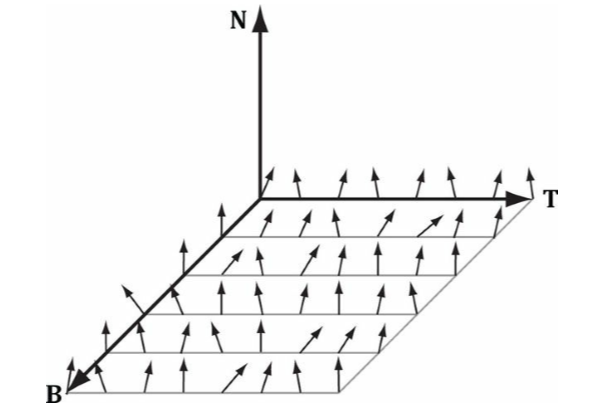
\includegraphics[width=0.8\textwidth]{images/normal_map_tnb.png}
    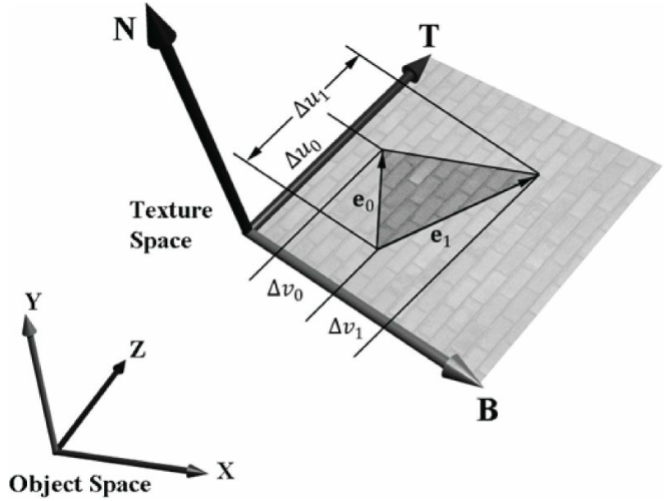
\includegraphics[width=0.8\textwidth]{images/normal_map_tnb_in_object_space.png}
\end{center}
假设三角形的三个顶点为$V_{0},V_{1},V_{2}$,对应的纹理坐标为$(u_{0},v_{0}),(u_{1},v_{1}),(u_{2},v_{2})$

\begin{gather*}
    \because \overrightarrow{e_{0}} = V_{1} - V_{0} \\ 
    \overrightarrow{e_{1}} = V_{2} - V_{0} \\ 
    \therefore (\Delta u_{0},\Delta v_{0}) = (u_{1} - u_{0}, v_{1} - v{0}) \\ 
    (\Delta u_{1}, \Delta v_{1}) = (u_{2} - u_{0}, v_{2} - v_{0}) \\ 
    \because \overrightarrow{e_{0}} = \Delta u_{0} \ast \overrightarrow{T} + \Delta v_{0} \ast \overrightarrow{B} \\
    \overrightarrow{e_{1}} = \Delta u_{1} \ast \overrightarrow{T} + \Delta v_{1} \ast \overrightarrow{B} \\
    \therefore \begin{bmatrix}
        \overrightarrow{e_{0}}.x & \overrightarrow{e_{0}}.y & \overrightarrow{e_{0}}.z \\ 
        \overrightarrow{e_{1}}.x & \overrightarrow{e_{1}}.y & \overrightarrow{e_{1}}.z  
    \end{bmatrix} = \begin{bmatrix}
        \Delta u_{0} & \Delta v_{0} \\ 
        \Delta u_{1} & \Delta v_{1}
    \end{bmatrix} \begin{bmatrix}
        \overrightarrow{T}.x & \overrightarrow{T}.y & \overrightarrow{T}.z \\ 
        \overrightarrow{B}.x & \overrightarrow{B}.y & \overrightarrow{B}.z  
    \end{bmatrix} \\ 
    \begin{bmatrix}
        \overrightarrow{T}.x & \overrightarrow{T}.y & \overrightarrow{T}.z \\ 
        \overrightarrow{B}.x & \overrightarrow{B}.y & \overrightarrow{B}.z  
    \end{bmatrix} = \begin{bmatrix}
        \Delta u_{0} & \Delta v_{0} \\ 
        \Delta u_{1} & \Delta v_{1}
    \end{bmatrix}^{-1} \begin{bmatrix}
        \overrightarrow{e_{0}}.x & \overrightarrow{e_{0}}.y & \overrightarrow{e_{0}}.z \\ 
        \overrightarrow{e_{1}}.x & \overrightarrow{e_{1}}.y & \overrightarrow{e_{1}}.z  
    \end{bmatrix} \\ 
    \because  \begin{bmatrix}
        \Delta u_{0} & \Delta v_{0} \\ 
        \Delta u_{1} & \Delta v_{1}
    \end{bmatrix}^{-1} = \frac{1}{\Delta u_{0} \Delta v_{1} - \Delta v_{0} \Delta u_{1}} \begin{bmatrix}
        \Delta v_{1} & -\Delta v_{0} \\ 
        -\Delta u_{1} & \Delta u_{0}
    \end{bmatrix} \\ 
    \therefore \begin{bmatrix}
        \overrightarrow{T}.x & \overrightarrow{T}.y & \overrightarrow{T}.z \\ 
        \overrightarrow{B}.x & \overrightarrow{B}.y & \overrightarrow{B}.z  
    \end{bmatrix} = \frac{1}{\Delta u_{0} \Delta v_{1} - \Delta v_{0} \Delta u_{1}} \begin{bmatrix}
        \Delta v_{1} & -\Delta v_{0} \\ 
        -\Delta u_{1} & \Delta u_{0}
    \end{bmatrix} \begin{bmatrix}
        \overrightarrow{e_{0}}.x & \overrightarrow{e_{0}}.y & \overrightarrow{e_{0}}.z \\ 
        \overrightarrow{e_{1}}.x & \overrightarrow{e_{1}}.y & \overrightarrow{e_{1}}.z  
    \end{bmatrix} 
\end{gather*}
通常直接传入每个顶点的法线和切线,可得到每个顶点在世界坐标系中的法线坐标和切线坐标值。N为顶点在世界坐标的法线,
则切线$T^{'} = T - (N \cdot T)N $,这样保证N与$ T^{'} $是正交的,则$B=N \times T^{'}$. 得到切线坐标系中的坐标值,
可以构造一个矩阵,将切线空间中的法线坐标变换到世界坐标,以得到法线坐标。
\begin{gather*}
    \begin{bmatrix}
        \overrightarrow{T}.x & \overrightarrow{T}.y & \overrightarrow{T}.z \\ 
        \overrightarrow{B}.x & \overrightarrow{B}.y & \overrightarrow{B}.z \\ 
        \overrightarrow{N}.x & \overrightarrow{N}.y & \overrightarrow{N}.z 
    \end{bmatrix}
\end{gather*}

\subsection{Height Map}
高度图是存储高度信息的数据,通常计算XY方向上的倾斜度

\begin{gather*}
    x_gradient = pixel(x-1,y) - pixel(x+1,y) \\
    y_gradient = pixel(x,y-1) - pixel(x,y+1) \\
    normalNew = normal + (U * x_gradient) + (V * y_gradient)
\end{gather*}

在的Bump Map\cite{CGPP3ed}中,有一个公式更加通用

\begin{align*}
    n^{'} = S(n + rt_{1} + gt_{2})
\end{align*}

它描述了两个方向上向量对法线的影响

\section{Texture Sampling}

前面说了纹理映射,如果是一一对应很好理解,找到对应的就行了,但现实中更复杂的是对特别小resolution低,
或特别大resolution高的产生的问题的处理。


\paragraph{low resolution}
纹理小会走样失真,需要一些图像处理技术来处理,
双线性插值Bilinear Interpolation是性价比很高的选择

\paragraph{high resolution}
纹理大会更走样失真,近处是锯齿Jaggies,远处是摩尔纹Moire。从信号的角度来看,就是采样频率过低无法还原信号源。
从透视的近大远小的原因,用远小的像素来表示面片的真实像素,自然会失真。

\paragraph{Upsampling}
上采样,
放大Magnification图像,基本是内插值方法,在原有像素点之间采样某种插值算法插入新的像素

\paragraph{Downsampling}
下(降)采样,
缩小Minification图像,把图像视口变小,原来多个像素的均值作为一个目标像素存储

\paragraph{Supersampling}
超采样,就是一个源像素大到一个区域事,把这个源像素细分为更多的子像素,获取子像素的采样,这种算法的计算量是几何倍数增长

\paragraph{Mipmap}
最理想的方法就是一一对应的查询,Mip comes from the Latin "multum in parvo", meaning a multitude in a small space.


\section{Color Space}
sRGB/RGB color space, linear/gamma space, 

设计师的眼睛与屏幕的显式因素


\chapter{Renderering}

在渲染方面上的研究与优化已经发展成熟,已成为一个非常复杂的系统了,本文的目标是从理解渲染的技术原理,从软渲染,到CPU,再到GPU。
为简化,我们以图元三角形为例,主要有两个阶段:
\begin{itemize}
    \item {决定那些像素坐标构成这个三角形}
    \item {决定这些像素的颜色值是多少,这个过程就是着色shading}
\end{itemize}
它们分别对应着图形学中另外两个概念,光栅化和光照模型。

\section{Rasterize}
光栅化
图形学中,是物理的三维世界,如何把三维物体在二维屏幕上显示,需要把它的三维属性都降为二维的结果,大致存在以下几个步骤:

\begin{itemize}
    \item {坐标变换}
    \item {属性计算,如颜色,纹理,alpha等}
    \item {光栅化}
\end{itemize}

\textsf{目前大众屏幕分辨率为1920x1080,在二维屏幕渲染时,内存中的FrameBuffer只保存着1920x1080个屏幕点的颜色,然后再映射到屏幕上面。
光栅化的,就是计算出1920x1080个点的颜色值的过程。把物体的数学描述转换为屏幕的像素值,是从连续到离散,即物理的坐标是浮点数,而屏幕坐标是整数,光栅化的过程是一个近似的过程。
在一些图形处理软件中就是把矢量图形转化成像素点的过程。}

\begin{description}
    \item [主动:] \textsf{定时渲染,与时间关系比较严格的}
    \item [被动:] \textsf{请求渲染,与动画相关的,以流畅为结果}
\end{description}

\text{目前处理光照生成图像的过程中,计算的级别有:}

\begin{itemize}
    \item {逐顶点光照,在每个顶点计算光照,在渲染图元内部进行插值,光照模型中的非线性关系会产生问题}
    \item {逐像素光照,Phong着色,在fragment对顶点法线进行插值}
\end{itemize}


\section{Photorealistic Rendering}

真实感图形技术包括消隐技术,光照模型,明暗处理和纹理,阴影生成等

\begin{itemize}
    \item {局部光照,仅处理光源直接照射物体表面的光照模型,与光栅化渲染算法相适应的,一次只考虑
    一个像素的光照强度,逐像素的光照计算,不能得到其他像素的光照影响值}
    \begin{itemize}
        \item {Lambert漫反射模型,不能很好处理镜面与高光}
        \item {Gourand}
        \item {Phong,支持高光与镜面}
        \item {Blinn-Phong,速度快,目前商业普遍使用}
        \item {Cook-Torrance,以双向反射的基础上}
    \end{itemize}
    \item {全局光照,基于光学物理原理,光照强度的计算依赖于光能在现实世界中的传播,考虑光线与整个场景中
    各物体表面以及物体表面之间的相互影响,包括多次反射、透射、散射等,成熟应用在离线渲染中}
    \begin{itemize}
        \item {光线跟踪,模拟光从光源出发经过若干次反射、折射达到摄像机的过程,由于只有最终到达摄像机的光线
        才对生成图像有贡献,实现中是以摄像机逆向发出光线,以寻求达到光源的路径。}
        \begin{itemize}
            \item {路径跟踪Path Tracing}
            \item {递归光线追踪Whitte-type}
            \item {分布式光线追踪Distrubution}
            \item {双向路径追踪Bidirectional Path}
            \item {Metropolis}
        \end{itemize}
        \item {辐射度算法,是一种物体空间的算法,用于解离散点或环境中表面曲面面片的光强度问题,而不是解图像平面
        投影的像素问题}
        \item {光子映射,改善漫反射辉映,焦散等全局光照效果,还无法应用在实时渲染中}
    \end{itemize}
\end{itemize}

\section{Non-Photorealistic Rendering}
对于某些场景,不需要真实感,需要一些艺术化的表现
钢笔素描的生成,
中国国画与书法的生成。
\newline
\textbf{Artistic Shading},艺术渲染,模拟人简画的素描之类的,是一种根据轮廓来来抽象效果。

\section{Image-Based Rendering}

IBR,基于图像的渲染,完全摒弃传统的先建模,然后确定光源的渲染方法,
它直接从一系列已知的图像中生成新颖的视口图像,适用于野外极其复杂场景的生成和漫游。

\section{Stereo Rendering}
立体渲染,是一种让人眼能够感受到立体效果的渲染方式,需要两个camera对同一个场景进行渲染,两个view得到
的图像略有差异(两个camera的投影矩阵的差异),让人产生深度的视觉效果。一般分左右两个camera。

通常渲染完成后,整张图像还需要一次后处理Barrel distortion桶形失真,以抵消VR设备固有的pincushion distortion枕形失真。
\begin{figure}[h]
    \centering
    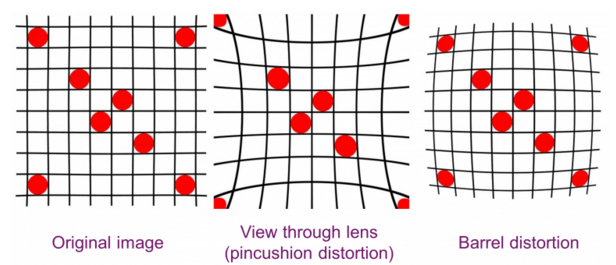
\includegraphics[width=\textwidth]{images/Optimising-OpenGL-ES-for-mobile-VR-lens-distortion.png}
    \caption{Phong Shading Model}
\end{figure}

\chapter{Illumination Model}

当光照射到物体表面时,物体会对光发生反射、透射、吸收、衍射、折射、干涉等。其中被物体吸收的部分转化为热。
反射、透射的光会进入人的视觉系统,使我们看见物体。为了模拟仿真这一真实的现象,建立一些数学模型来替代复杂的真实
物理模型,这些模型就称为光照模型。

\section{Lamertian}
1970年Bouknight提出了第一个光反射模型。1971Gourand提出“漫反射模型+插值”的思想,称为Gourand明暗处理。
即出物体表面朝向(即法线)是确定物体表面上一点光强的主要因素,用Lambert漫反射定律计算物体表面上各多
边形的光强,对光照射不到的使用环境光代替。
\textbf{Lambert's cosin law},告诉我们曲面表面的颜色c与表面法线和光源方向的夹角的余弦值cosine成正比。

\begin{align*}
c \propto cos(\theta) \\
c \propto n \cdot l 
\end{align*}

漫反射:当光线从光源照射到曲面表面时,表面向每个方向散射辐射量。漫反射符合兰伯特定律。

\begin{align*}    
c_{diffuse} = max(0, \hat{n} * \hat{l}), \\
c_{ambient} = Kd * Ia, \\
c_{light} = Kd * Il, \\ 
c_{final} = c_{ambient} + c_{light}c_{diffuse}, \\
0 < Kd < 1, 
\end{align*}

Kd是材质对环境光的反射系数,Ia表示环境光强度,Il表示点光源强度
注意,这里存在一个前提,就是假设光源方向l不依赖渲染物体的位置信息,就是光与渲染对象有足够的远,就是
方向光directional light。

\section{Phong Model}

Phong模型引入镜面光,即ADS(ambient,diffuse,specular),认为镜面与反射的光强和反射光线与视线的夹角相关

\begin{figure}[htbp]
    \centering
    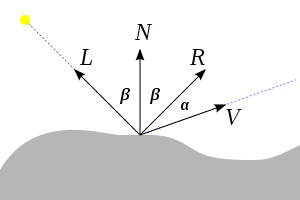
\includegraphics[width=0.8\textwidth]{images/phong-shading-model.png}
    \caption{Phong-Model-Specular}\label{Phong-Model-Specular}
\end{figure}

图\ref{Phong-Model-Specular}中的$\alpha$ 很小时,就是高光效果

\begin{align*}
    R = -L + 2(L \cdot N) * N \\
    I_{spec}=Ks * Il * (dot(V, R))^N_{s}
\end{align*}

Ks为镜面反射系数,Ns为高光指数。

\begin{figure}[htbp]
    \centering
    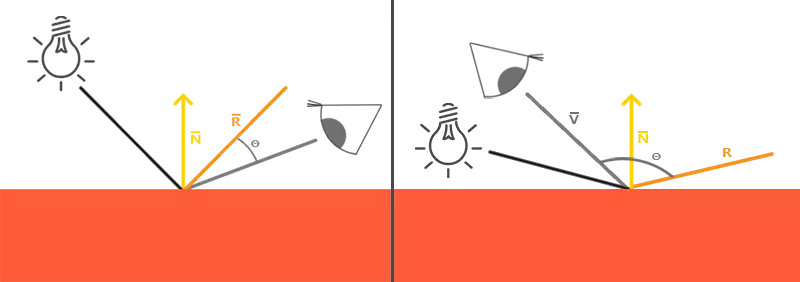
\includegraphics[width=0.8\textwidth]{images/classical-phong.png}
    \caption{Phong-Problem}\label{Phong-Problem}
\end{figure}
图\ref{Phong-Problem}模型中存在一个问题就是$\alpha$的角度大于90度时,会导致结果为负,产生假象。

Blinn-Phong是基于Phong的修正模型,

\begin{figure}[htbp]
    \centering
    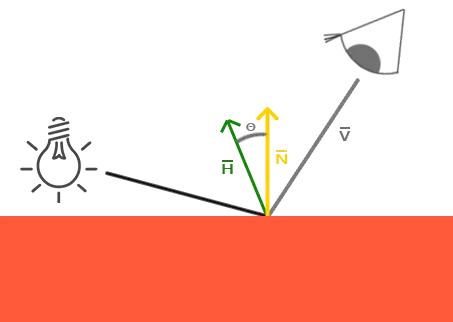
\includegraphics[width=0.8\textwidth]{images/blinn-phong.png}
    \caption{Blinn-Phong}\label{Blinn-Phong}
\end{figure}

图\ref{Blinn-Phong}通过半角来方法来解决可能出现角度大于90度的问题。

\begin{align*}
    H = \frac{L + V}{|L + V|}, \\
    I_{spec} = Ks * Il * (dot(N, H))^N_{s}
\end{align*}

H是入射光线方向L与视线方向V的中间向量,称之为半角向量。Classical-Phong更真实,Blinn-Phong高光更柔和,且计算速度较快,
实际中应用更广,OpenGL和DirectX渲染管线中是默认渲染模型。

\section{Global Illumination}
现实中的物体表面会接收大部分或全部来自其他反射出来的光线,称为indirect lighting或mutual illumination。
局部光照模型只考虑光对物体的照明,忽略了物体间的相互影响,其一般公式可以表示为

\begin{align*}
    I = I_{abmient} + \sum_{i}^{N}I_{light}\frac{1}{k_{c}+k_{l} \cdot d_{i} + k_{q} \cdot d_{i}^2}
    \left[ k_{d}(N \cdot L) + k_{s}(R \cdot V)^n \right]
\end{align*}

每个光源对物体的影响主要包括漫反射和镜面反射两部分,局部照明的阴影算法需要单独考虑。
\newline
全局照明考虑更全面,它自带阴影效果。它主要有两种算法:
\begin{itemize}
    \item {光线追踪法, 关注于镜面反射光,可严格追踪反射光线的方向,实际中采用逆向追踪法,减少计算量}
    \item {辐射度法, 关注于漫反射光,}
\end{itemize}
基本模型是 
\newline

\begin{align*}
    I_r = I_{ia}R_{a} + \sum_{l}I_{il}(N \cdot L_{l})d \omega_{il}(sR_{s} + dR_{d})
\end{align*}

其中的环境光和漫反射分量不依赖于观察者的位置View's Position。假设表面是由微面元组成microfacet,其镜面分量为:
\newline

\begin{align*}
    R_s = \frac{F}{\pi} \frac{DG}{\pi (N \cdot L)(N \cdot V)}
\end{align*}

为更加丰富,引入了几何项G,Fresnel项F,粗糙度项D。
\newline

\textbf{粗糙度项D},代表了可以有效反射光的那一部分微面元所占的比例,有多种分别函数。
高斯分布模型
\newline

\begin{align*}
    D = ce^{-(\alpha / m)^2}
\end{align*}

Bechmann分布函数
\newline

\begin{align*}
    D = \frac{1}{m^2cos^4(\theta)}e^-(tan\alpha / m)^2
\end{align*}

\textbf{几何项G},几何衰减项,表现了微小面元之间的互相遮挡shadowing and masking所造成的影响。
\newline

\begin{align*}
    G = \left\{
        1, \frac{2(N \cdot H)(N \cdot V)}{(V \cdot H)}, \frac{2(N \cdot H)(N \cdot L)}{(V \cdot H)} 
    \right\}
\end{align*}

\textbf{Fresnel项F},描述了在每一个微面元上光是如何反射,与入射角和波长相关。
\newline

\begin{align*}
    c = cos(\theta) = V \cdot H \\
    g^2 = n^2 + c^2 - 1 \\
F = \frac{1(g-c)^2}{2(g+c)^2} \left\{ 1+\frac{[c(g+c)-1]^2}{[c(g-c)+1]^2} \right\}
\end{align*}

\section{Physically based Rendering}

PBR refers to the concept of using realistic shading/lighting models along with measured surface values to accurately represent real-world materials

\chapter{Texture}

可阅读
Chapter 20 Textures and Texture Mapping\cite{CGPP3ed}

Chapter 11 Texture Mapping\cite{FCG4ed}

Chapter 6 Texturing\cite{RTR4ed}

纹理应用在表面的大致逻辑是
\begin{lstlisting}
    Color texture_lookup(Texture t, float u, float v) {
        int i = round(u * t.width() - 0.5);
        int j = round(v * t.height() - 0.5);
        return t.get_pixel(i,j);
    }
    Color shade_surface_point(Surface s, Point p, Texture t) {
        Vector normal = s.get_normal(p);
        (u,v) = s.get_texcoord(p);
        Color diffuse_color = texture_lookup(t, u, v);
        // compute shading using diffuse_color and normal 
        // return shading result    
    }
\end{lstlisting}

\section{Texture Coordinate}
 纹理坐标的生成.

以顶视图Y轴方向来看,对X(S)和Z(T)生成对应的纹理坐标值UV,即Y平面为UV展开

\begin{enumerate}
    \item \textsf{遍历所有点得到lowestX和highestX,lowestX=-12.00,highestX=134.56}
    \item \textsf{得到绝对范围 range=(lowest - highest) * -1 = (-12.00-134.56)*-1=146.56}
    \item \textsf{与0的偏移值offset=0-lowestX=0 - (-12.00)=12}
    \item \textsf{vertex x=87.45, absoluteX=X+offset=87.45+12=99.45}
    \item \textsf{get S value, s = absoluteX / range = 99.45/145.56=0.679}
    \item \textsf{do the same for Z axis to get T value}
\end{enumerate}

由Image Space得到Texture space T, 存在一个函数映射Surface S in World space, 数学模型如下:

\begin{align*}
    \phi &: S \rightarrow T \\
    &: (x,y,z) \rightarrow (u,v)
\end{align*}

函数$\phi$存在很多种形式

\subsection{Planar Projection}

orthographic viewing $M_{t}$是变换矩阵

\begin{align*}
    \phi(x,y,z) = (u,v) \qquad where 
    \begin{bmatrix} u \\ v \\ * \\ 1 \end{bmatrix} = M_{t} 
    \begin{bmatrix} x \\ y \\ z \\ 1 \end{bmatrix}
\end{align*}

perspective viewing $P_{t}$是投影矩阵

\begin{align*}
    \phi(x,y,z) = (u/w,v/w) \qquad where 
    \begin{bmatrix} u \\ v \\ * \\ w \end{bmatrix} = P_{t} 
    \begin{bmatrix} x \\ y \\ z \\ 1 \end{bmatrix}
\end{align*}


\subsection{Sphereical Coordinates}

\begin{equation}
    \phi(x,y,z) = ([\pi+atan2(y,x)]/2\pi,[\pi-acos(z/s\|x\|)]/\pi)
\end{equation}

\subsection{Cylindrical Coordinates}

\begin{align*}
    \phi(x,y,z) = (\frac{1}{2\pi}[\pi+atan2(y,x)]/2\pi,\frac{1}{2}[1+z])
\end{align*}

\subsection{Cubemaps}

\begin{align*}
    \phi(x,y,z) \mapsto (\frac{x}{z},\frac{y}{z})
\end{align*}

\subsection{Interpolated Texture Coordinates }

\begin{description}
    \item [distortion] \textsf{映射关系是一个连续的函数,就存在失真,扭曲,畸变}
    \item [seam] \textsf{拓扑可以展开为平面,但是因为顶点可能有多个uv值,会出现缝隙问题,边界过渡问题}
\end{description}

\subsection{UV Unwrapping}

UV展开就是把物体的表面映射到平面图像上的过程。为了让弯曲的表面信息也能在平面上被精准存放下来,对切割线seam的要求

\section{Bump Map}

为增加表面法向量细节,如一个平面法向量处处相同,即时使用纹理,光照效果仍然不够真实,可以增加扰动表面面皮的法向量,
从而形成比较真实的效果。

纹理贴图存储的是颜色值,而Bump Map存储的是凹凸数据,通常是高度值。
Bump Map是Phong Shading的一项扩展,因为表面法线用来计算顶点的光亮,而Bump Map就是为了影响法线的改变,最终影响颜色值。
所以算是一种负责光方向的纹理映射,不同的凹凸数据,使用不同的方法来影响法线。

\begin{itemize}
    \item \text{Emboss Bump Map}
    \item \text{DOT3 Bumap Map}
\end{itemize}

\subsection{Normal Map}

是实时渲染中,通常使用凹凸贴图的变种法线贴图,bluish texture偏蓝色纹理,法线贴图在纹理的每个像素中存储一个颜色。
有两种方法生成法线贴图
\paragraph{灰度图}
预先计算每个像素与其垂直和水平相邻像素之间的差别,将两个结果数字(导数)转换为单位法线并存储为颜色
\paragraph{精模烘焙法线}
把纹理的每个像素与精模的表面位置结合起来,将其结果编码为法线存储为颜色值

为使生成的纹理可以在任意旋转下均反复使用,存储的法线必须在\textbf{切线空间}中,切线空间由三个向量normal法线,tangent切线,binormal副法线组成。
切线空间决定了表面的朝向。

切线空间的映射依赖物体的UV纹理,因为UV纹理中的决定世界空间中的切线空间的两个向量,切线和副法线。
生成较好的UV纹理在切线空间中不穿帮是比较困难和耗时的。

\begin{center}
    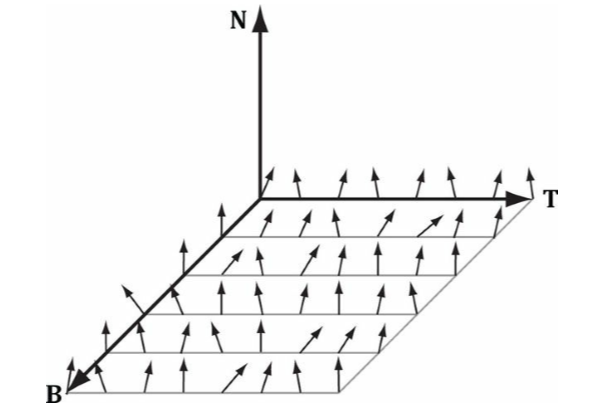
\includegraphics[width=0.8\textwidth]{images/normal_map_tnb.png}
    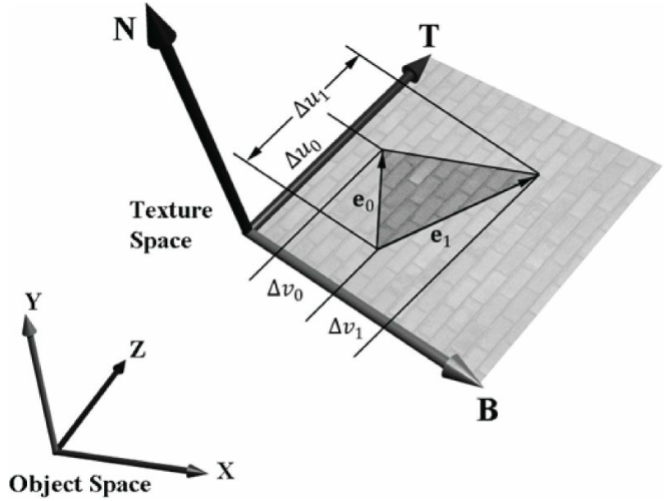
\includegraphics[width=0.8\textwidth]{images/normal_map_tnb_in_object_space.png}
\end{center}
假设三角形的三个顶点为$V_{0},V_{1},V_{2}$,对应的纹理坐标为$(u_{0},v_{0}),(u_{1},v_{1}),(u_{2},v_{2})$

\begin{gather*}
    \because \overrightarrow{e_{0}} = V_{1} - V_{0} \\ 
    \overrightarrow{e_{1}} = V_{2} - V_{0} \\ 
    \therefore (\Delta u_{0},\Delta v_{0}) = (u_{1} - u_{0}, v_{1} - v{0}) \\ 
    (\Delta u_{1}, \Delta v_{1}) = (u_{2} - u_{0}, v_{2} - v_{0}) \\ 
    \because \overrightarrow{e_{0}} = \Delta u_{0} \ast \overrightarrow{T} + \Delta v_{0} \ast \overrightarrow{B} \\
    \overrightarrow{e_{1}} = \Delta u_{1} \ast \overrightarrow{T} + \Delta v_{1} \ast \overrightarrow{B} \\
    \therefore \begin{bmatrix}
        \overrightarrow{e_{0}}.x & \overrightarrow{e_{0}}.y & \overrightarrow{e_{0}}.z \\ 
        \overrightarrow{e_{1}}.x & \overrightarrow{e_{1}}.y & \overrightarrow{e_{1}}.z  
    \end{bmatrix} = \begin{bmatrix}
        \Delta u_{0} & \Delta v_{0} \\ 
        \Delta u_{1} & \Delta v_{1}
    \end{bmatrix} \begin{bmatrix}
        \overrightarrow{T}.x & \overrightarrow{T}.y & \overrightarrow{T}.z \\ 
        \overrightarrow{B}.x & \overrightarrow{B}.y & \overrightarrow{B}.z  
    \end{bmatrix} \\ 
    \begin{bmatrix}
        \overrightarrow{T}.x & \overrightarrow{T}.y & \overrightarrow{T}.z \\ 
        \overrightarrow{B}.x & \overrightarrow{B}.y & \overrightarrow{B}.z  
    \end{bmatrix} = \begin{bmatrix}
        \Delta u_{0} & \Delta v_{0} \\ 
        \Delta u_{1} & \Delta v_{1}
    \end{bmatrix}^{-1} \begin{bmatrix}
        \overrightarrow{e_{0}}.x & \overrightarrow{e_{0}}.y & \overrightarrow{e_{0}}.z \\ 
        \overrightarrow{e_{1}}.x & \overrightarrow{e_{1}}.y & \overrightarrow{e_{1}}.z  
    \end{bmatrix} \\ 
    \because  \begin{bmatrix}
        \Delta u_{0} & \Delta v_{0} \\ 
        \Delta u_{1} & \Delta v_{1}
    \end{bmatrix}^{-1} = \frac{1}{\Delta u_{0} \Delta v_{1} - \Delta v_{0} \Delta u_{1}} \begin{bmatrix}
        \Delta v_{1} & -\Delta v_{0} \\ 
        -\Delta u_{1} & \Delta u_{0}
    \end{bmatrix} \\ 
    \therefore \begin{bmatrix}
        \overrightarrow{T}.x & \overrightarrow{T}.y & \overrightarrow{T}.z \\ 
        \overrightarrow{B}.x & \overrightarrow{B}.y & \overrightarrow{B}.z  
    \end{bmatrix} = \frac{1}{\Delta u_{0} \Delta v_{1} - \Delta v_{0} \Delta u_{1}} \begin{bmatrix}
        \Delta v_{1} & -\Delta v_{0} \\ 
        -\Delta u_{1} & \Delta u_{0}
    \end{bmatrix} \begin{bmatrix}
        \overrightarrow{e_{0}}.x & \overrightarrow{e_{0}}.y & \overrightarrow{e_{0}}.z \\ 
        \overrightarrow{e_{1}}.x & \overrightarrow{e_{1}}.y & \overrightarrow{e_{1}}.z  
    \end{bmatrix} 
\end{gather*}
通常直接传入每个顶点的法线和切线,可得到每个顶点在世界坐标系中的法线坐标和切线坐标值。N为顶点在世界坐标的法线,
则切线$T^{'} = T - (N \cdot T)N $,这样保证N与$ T^{'} $是正交的,则$B=N \times T^{'}$. 得到切线坐标系中的坐标值,
可以构造一个矩阵,将切线空间中的法线坐标变换到世界坐标,以得到法线坐标。
\begin{gather*}
    \begin{bmatrix}
        \overrightarrow{T}.x & \overrightarrow{T}.y & \overrightarrow{T}.z \\ 
        \overrightarrow{B}.x & \overrightarrow{B}.y & \overrightarrow{B}.z \\ 
        \overrightarrow{N}.x & \overrightarrow{N}.y & \overrightarrow{N}.z 
    \end{bmatrix}
\end{gather*}

\subsection{Height Map}
高度图是存储高度信息的数据,通常计算XY方向上的倾斜度

\begin{gather*}
    x_gradient = pixel(x-1,y) - pixel(x+1,y) \\
    y_gradient = pixel(x,y-1) - pixel(x,y+1) \\
    normalNew = normal + (U * x_gradient) + (V * y_gradient)
\end{gather*}

在的Bump Map\cite{CGPP3ed}中,有一个公式更加通用

\begin{align*}
    n^{'} = S(n + rt_{1} + gt_{2})
\end{align*}

它描述了两个方向上向量对法线的影响

\section{Color Space}
sRGB/RGB color space, linear/gamma space, 

设计师的眼睛与屏幕的显式因素

\chapter{Shadow}

可参考Advanced Lighting\cite{LearnOpenGL}

\section{Shadow Map}

创建阴影的步骤:
\paragraph{一} 
以光源为视点,投影渲染整个场景,得到深度图ShadowMap并保存变换矩阵。ShadowMap中以光源为视点
时,所有可视点的深度。注意投影的区别:如果是DirectionLight则是正交投影,如果是PointLight,SpotLight则是透视投影

\paragraph{二}
以相机为视点渲染,对场景中的每个顶点,将其变换到以光源为视点的空间,若其深度大于ShadowMap中对应点
深度值,说明光源射来的光线被物体遮挡了,则该点处于阴影中。

运用渲染到纹理方法render to target,以场景中的光源为坐标原点,建立光源坐标系,就是场景深度
把render target(一般是R32F的surface)就是Shadow Map。 

接着正常render frame buffer, 启用depth buffer,将场景中的世界坐标的物体转化到以光源为基准的
投影坐标系中

世界坐标 $\rightarrow$ 物体坐标 $\rightarrow$ 光源坐标 $\rightarrow$ 光源视图坐标 $\rightarrow$ 光源投影坐标

任何在fragment shader中比较深度值,深度值小于shadow map对应的深度,就是光源照射地方,否则就是照射不到地方。
比较深度值时要把坐标转换为窗口坐标,因为shadow map是render to target的surface的结果。

\begin{itemize}
    \item [优点] \text{不用像volume那样去计算所有对象形状,只产生一直map}
    \item [缺点] \text{阴影有锯齿,比较深度值时就两种值,有阴影1和无阴影0,在阴影的边缘0和1交替出现而产生锯齿}
\end{itemize}

\paragraph{Shadow acne}
\begin{center}
    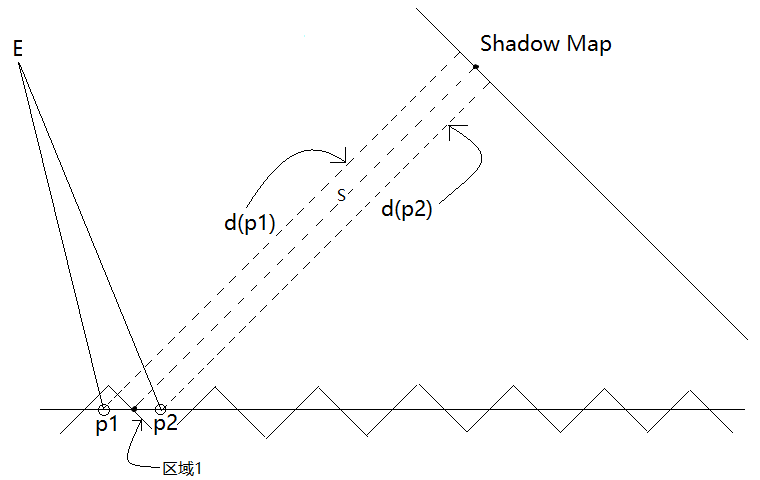
\includegraphics[width=0.4\textwidth]{images/shadow_acne.png}
    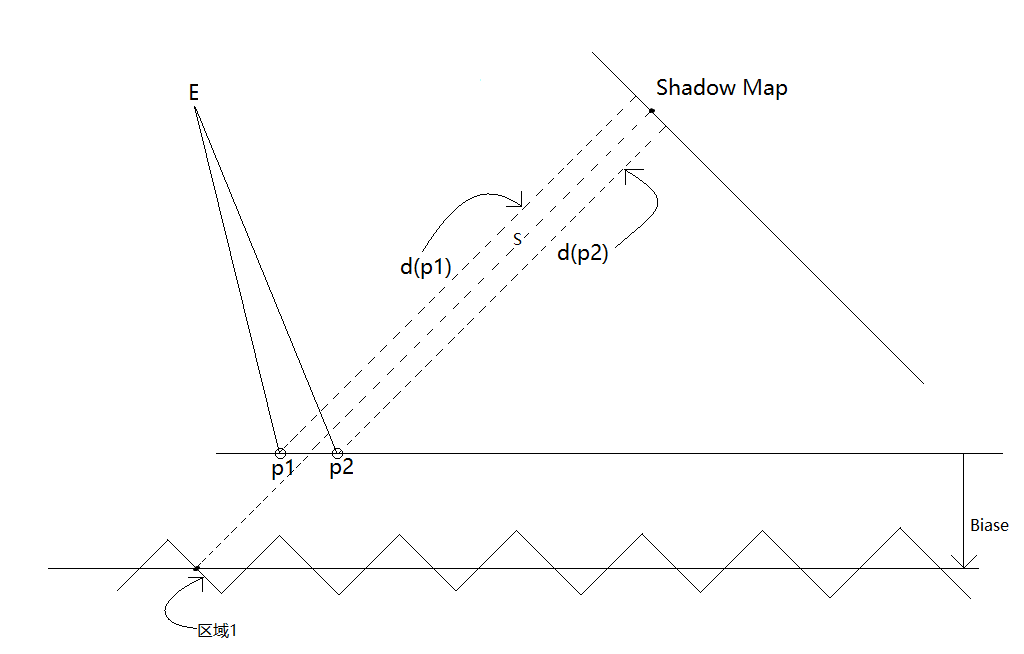
\includegraphics[width=0.4\textwidth]{images/shadow_acne_offset.png}
\end{center}
ShadowMap的分辨率有限,很容易产生阶梯状的边缘,每个Texel对应场景中的一个区域,如左边的图,点$p_{1}$和$p_{2}$对应屏幕上
不同的点,有$d(p_{1})>s, d(p_{2})<2$,点$p_{1}$也处在阴影中,解决的办法就是给shadow map中的深度值进行一个常量的偏移。

当三角形相对于光源而言,斜率过大,就需要一个非常大的偏移,就出现如下图所示的效果
\paragraph{Shadow Peter-pinning}
\begin{center}
    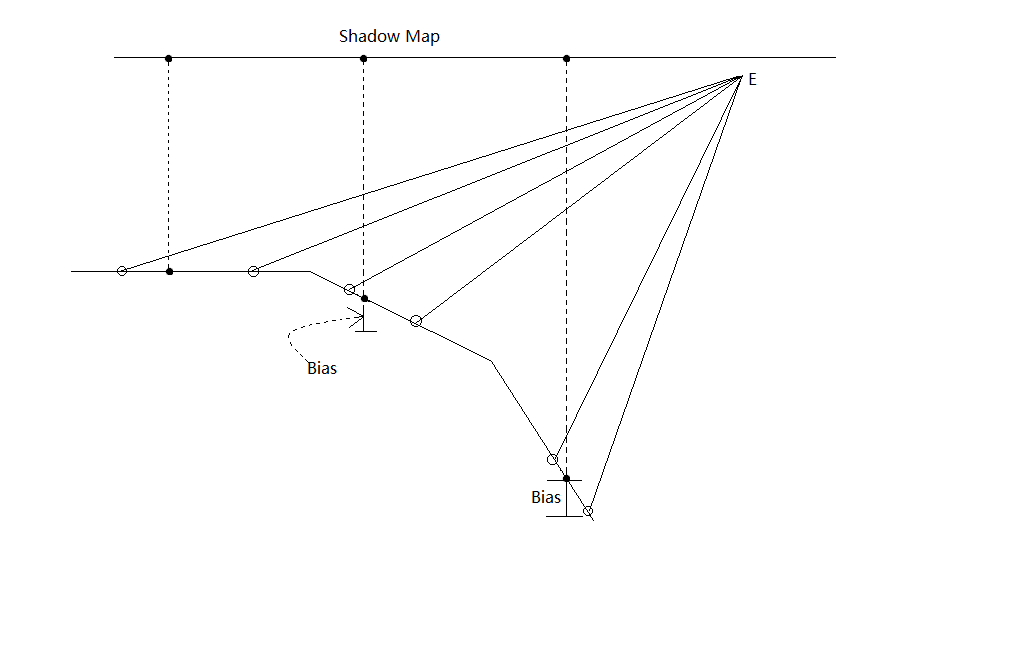
\includegraphics[width=0.8\textwidth]{images/shadow_peter-pinning.png}
\end{center}
为解决这种问题,图形显卡通过一种slope scaled bias的光栅化状态进行内置支持。

\paragraph{Shadow Bias}

\begin{gather*}
    bias = factorSlope \times slope + constantBias
\end{gather*}

\section{Hard \& Soft}
生成的阴影,其边缘没有过渡的,就会产生锯齿现象,而现实世界中的阴影边缘过渡得渐变很明显。
无渐变的shadow称为Hard Shadow,有渐变的称为Soft Shadow。为了产生渐变,就不能简单进行比较判断,得到是否的结果,
这就是shadow filtering的内容。

PCF(Perecentage Closer Filter), 将深度比较的结果0和1存储在一个render target里面,然后对其进行过滤操作,
产生值为0.2,0.5,...等灰度值的,即soft shadow。消耗时间较长,就简化成横向或纵向过滤,减少采样数量。

CSM(convolution shadow map), 此方法基于阴影重建,深度值比较的结果要么是1,要么是0,从而构造一个x坐标为[-1,1],
y坐标为[0,1]的函数,对函数进行FFT变换,运用基准函数sin和cos来重新构建shadow map。 

VSM(variance shadow map), 此方法应用切尔雪夫不等式,

\section{Perspective Aliasing}
近处锯齿现象,shadow map的分辨率不够。在camera视角下,近处的分辨率较高,一小片段对应着大量的pixel,而光源视角下的shadow map精度
并没有发生改变,就会大量的pixel对应着同一点,因而产生锯齿。 解决方案就是CSM(Cascaded Shadow Map),即一张不够,就多张来,
可参考微软的CSM\cite{CSM-msdn}


\chapter{Algorithm}
记录一些算法和思路

\section{Camera}

\begin{figure}[h]
    \centering
    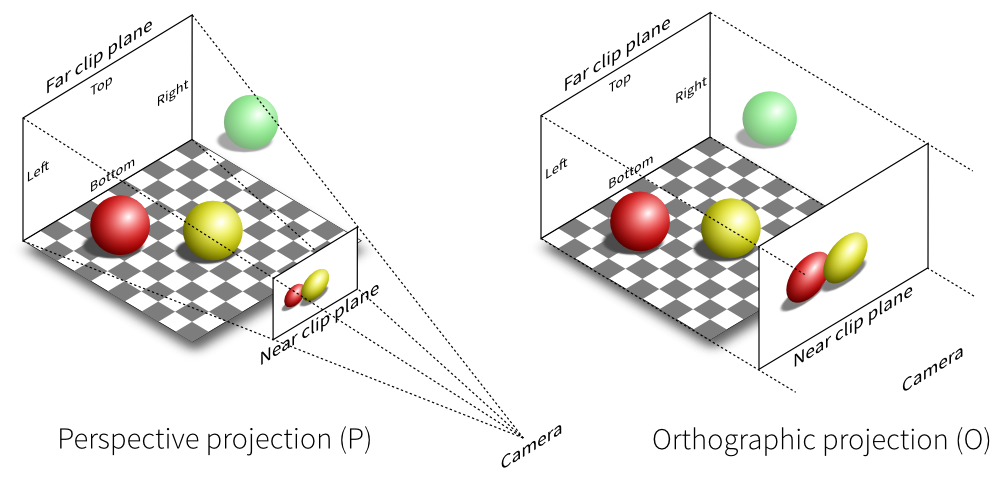
\includegraphics[width=1\textwidth]{images/camera-perspective-and-orthographic.png}
    \caption{左边:透视投影;右边:右边正交投影}    
\end{figure}

\subsection{Perspective Best-Fit}
关于camera的自动对焦算法,对透视camera有: side是bounding box的最大边, distance是从camera的位置到bounding box的中心距离

\begin{align*}
    tan(\alpha / 2) = \frac{(side / 2)}{distance}
\end{align*}

对应的threejs的代码如下:

\begin{lstlisting}
    let box = calculateBoundingBoxInScene();
    let center = new THREE.Vector3(), size = new THREE.Vector3();
    box.getCenter(center); box.getSize(size);
    let maxSide = Math.max(size.x, Math.max(size.y, size.z));    
    let distance = maxSide /
         ( 2 * Math.tan(THREE.Math.DEG2RAD * alpha / 2));  
    camera.position.set(center.x, center.y, center.z - distance);
    camera.position.z *= Math.sqrt(3);
\end{lstlisting}

\subsection{Perspective Side}



\section{ Edge Function }
Juan Pineda \cite{EdgeFunction} 在他论文提出的概念,就是\textbf{barycentric coordinates}的应用。
它在计算三角形属性方面上有很大的优势,如深度z-depth、颜色color、纹理坐标uv、法线等插值计算。
重心(质心)坐标的应用主要体现在:
\begin {itemize}
    \item {判断一个点是否在三角形内}
    \item {根据三角形三个顶点得到三角形内一个点P}
\end {itemize}
在软光栅化或光线追踪都用得到。

\begin{figure}[h]
    \centering
    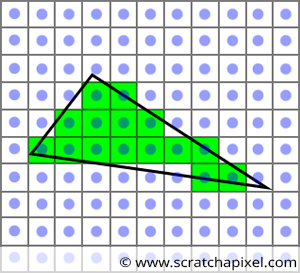
\includegraphics[width=0.25\textwidth]{images/rasterization-triangle1.png}
    \hspace{0.1cm}
    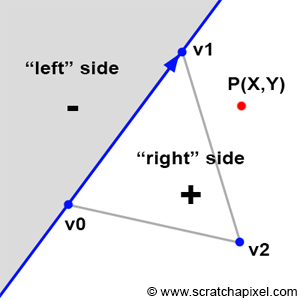
\includegraphics[width=0.25\textwidth]{images/rasterization-triangle2.png}
    \hspace{0.1cm}
    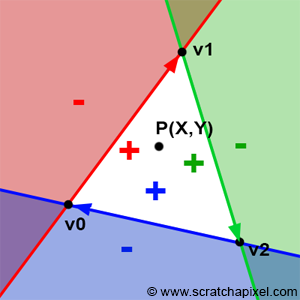
\includegraphics[width=0.25\textwidth]{images/rasterization-triangle3.png}
    \caption{左边:测试像素是否覆盖三角形,是光栅化算法的原理;
    中间:判断点与线的关系,大于0在右边,小于0在左边,等于0在线上;
    右边:在白色区域中的点都是位于三角形边的右边
    }    
\end{figure}
遍历整个FrameBuffer去判断点是不是在在三角形内部,太浪费时间去遍历不可能的结果了。
\begin{figure}[h]
    \centering
    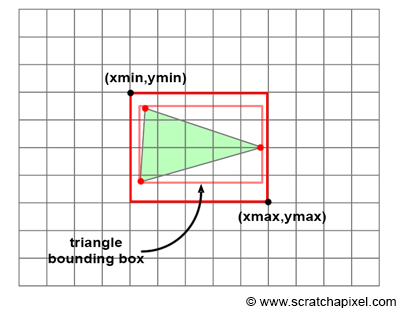
\includegraphics[width=0.3\textwidth]{images/rasterization-boundingbox.png}
    \caption {三角形的顶点告诉了大致范围,减少遍历的次数,提高访问性能}
\end{figure}
计算boundingbox的算法很简单,速度也快。

\section{Reconstructing Position From Depth}
需求:根据当前像素的Depth计算出View空间中的Position
先分析depth是如何计算出来的,在vertex shadeer中
\begin{lstlisting}
    outPos = mul(inPos, mvp);
    outDepth.xy = outPos.zw;
\end{lstlisting}
在pixel shader中,
\begin{lstlisting}
    depth = outDepth.x / outDepth.y;
\end{lstlisting}
按照这个过程逆运算回去
\begin{lstlisting}
    z = texture(depthSampler, inUV);
    x = inUV.x * 2 - 1;
    y = (1 - inUV.y) * 2 - 1;
    pos = (x,y,z,1)
    pos = mul(pos, mvpInverse);
    pos = pos.xyz / pos.w;
\end{lstlisting}
但是存在一些问题
\begin{itemize}
    \item {z/w是非线性分布的,经过RTT(Render To Texture)后再变换回去,精度存在误差}
    \item {计算量大}
\end{itemize}
从物理状态来看看摄像机的视锥体的抽象形式,从摄像机位置到远裁剪面发射一条射线,存在一个关系:

\begin{figure}[h]
    \centering
    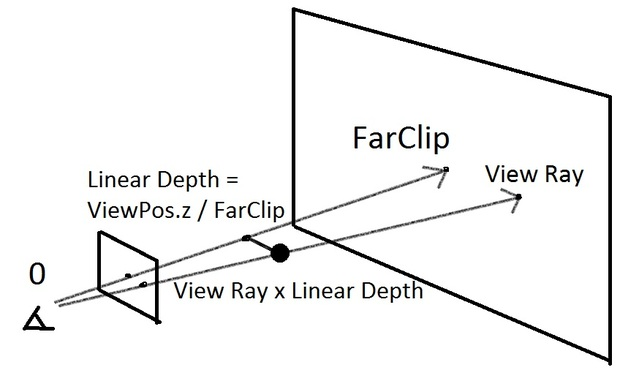
\includegraphics[width=0.5\textwidth]{images/reconstructing-position-from-depth.png}
\end{figure}

\begin{lstlisting}
    posView = viewRayDir * linearDepth;    
    linearDepth = posView.z / farClipDistance;
\end{lstlisting}

linearDepth是规格化的Z值,它满足线性分布。现在的问题就如何得到RayDir向量了。在View空间中,摄像机的位置是(0,0,0),
对于可见的每个点,从摄像机出发的射线都与远裁剪面相交,交点就是方向向量RayDir的坐标。由图中可知,是利用中心线和射线组成的三角形,满足等比关系,是线性关系。
远裁剪面的四个顶点是可以计算出来的,思路就出来了。

\begin{itemize}
    \item {1. 把posView.z/farClipDistance的值保存到RTT中,得到的值满足线性关系}
    \item {2. 从RTT中得到linearDepth, 从vertex shader中得到viewRayDire.xy, }
\end{itemize}

\begin{lstlisting}
    viewRayDir = float3(farClip.x, farClip.y, farClipDistance);
    posView = viewRayDir * linearDepth;
\end{lstlisting}

\section{Control}

场景中使用控件来改变形态,存在两种方法,一是改变object的旋转,非常适合单一场景中的物体;一是漫游之类的控件,改变camera的
形态来对静态的模型进行观察,多用于大场景中,如游戏中,有其他参考物的可以使用这种方式。

\subsection{Trackball}
轨迹球\cite{Trackball}
轨迹球就是在屏幕之外虚构一个球形曲面,使鼠标在二维屏幕上的移动投影到球形曲面上。
即一个半球覆盖在屏幕上面。以屏幕中心为球心O,X轴向右,Y轴向上,Z轴向外。当鼠标在球面的范围内移动时,可以由二维屏幕上的二维左边点P(x,y),通过数学关系求得其在球面上的投影点P'。
鼠标从P1移动到P2,对应的球面就是从P1'到P2'。产生两个向量V1=OP1',V2=OP2',  
V1与V2的叉乘得到向量N,即三维物体的旋转轴,V1到V2的转角量就是三维物体的旋转角度。
屏幕时矩形,球形的投影在屏幕的平面上只会是一个圆,总会有些区域的点投影后会落在球面之外。


\section{Grid}
绘制网格,是很多场景都需要的,有两种思路, 基于直线,基于Pattern网格思路。
直线的思路就是一个plane效果。而Pattern的网格思路是一个模式,更符合screen效果。
\begin{lstlisting}
    uniform vec2 pitch; // unit-x, unit-y
    uniform float scale; // 10

    float offsetX = gl_FragCoord.x;
    float offsetY = 1.0 - gl_FragCoord.y;
    if (int(mod(offsetX, pitch[0])) == 0 || int(mod(offsetY, pitch[1])) == 0) {
        if (int(mod(offsetX, pitch[0] * scale)) == 0 || int(mod(offsetY, pitch[1] * scale)) == 0) {
            gl_FragColor = vec4(0.8, 0.8, 0, 0.5);
        } else {
            gl_FragColor = vec4(0.8, 0, 0, 0.5);
        }
    } else {
        discard;
    }
\end{lstlisting}


\chapter{API}

\section{Shader}

\subsection{screen space derivative}
屏幕空间偏导数
GPU always evaluate fragment/pixel shaders on 2x2 blocks of pixels at a time.

use this techniques for rendering antialiased lines

\begin{figure}[h]
    \centering
    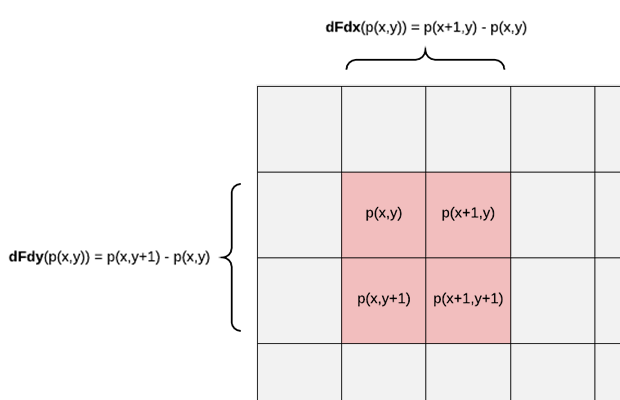
\includegraphics[width=\textwidth]{images/Shader-Derivatives.png}
\end{figure}

antialiasing,AA抗锯齿,对于一张纹理,给定UV坐标后,不仅仅是直接采样,还要考虑周围方形
区域内采样的结果,这个区域就是ddx和ddy给定的区域,在shader中调用texture时,后台进行了处理,
在一些高级的profiles中,还是允许自定义滤波窗口大小的

mipmap,在屏幕空间中,纹理坐标变换剧烈,Derivatives are used during texture sampling to
select the best mipmap level.

\subsubsection{fwidth}
GLSL中,fwidth函数返回的是X和Y方向偏导数的绝对值的和,而单方向的偏导数可以通过ddx和ddy获得

注意,这些函数与像素有关,只能在fragment/pixel shader中使用

\section{Vulkan}

vulkan是控制GPU设备的API,相比OpenGL,由OpenGL驱动提供的功能都需要自己实现,包括,同步,进度,内存管理等。
所以vulkan是适合大型复杂的图形渲染,定制性要求很高,OpenGL提供不了的功能。

\subsection{Resource}

vulkan的操作基于数据,所有data都存储在resources中,它们被后台内存管理着,构建这些资源大致有两步
\begin{itemize}
    \item {resource is created, ex, vkCreateBuffer}
    \item {resource needs to be backed by memory, 允许应用程序管理内存}
\end{itemize}

\subsubsection{buffers}

线性存储块,可拥有存储任何的数据,它同样可以存储图像数据

\subsubsection{images}

图像,具有结构性,类型,格式的固定数据

\section{3D Render Library}

\subsection{OpenSceneGraph}

\subsection{bgfx}

\subsection{three.js}

\subsection{Babylon.js}

\chapter{Physical Terminology}

\section{anisotropy}
各向异性或非均向性,指物体的全部或部分属性性质随方向的不同有不同的变化

在计算机图形学中,各向异性表面在围绕几何法线旋转时外观会发生变化。

任何具有细粒度的东西,会产生影响外观的作用。

\subsection{anisotropy reflect}
基于反射表面上存在的小凹槽或凸起,改变光源照射物体的方向,反射在各个方向上具有不同的特性。

可用来平滑图像,克服高斯模糊的缺陷。

\subsection{isotropy reflect}
表面反射均匀具有模糊效果, 反射总是在与颗粒相反的方向拉伸。

\section{Light}

\subsection{Conception}

\subsubsection{Absorption \& Scattering}

吸收与散射, 当光在一个不均匀介质中或半透明的材质中传播时,会被吸收或散射。

\subsection{Refraction}

\subsubsection{IOR}
index of refraction,折射率,光在真空中的传播速度与光在介质中的传播速度之比。
折射率与介质的电磁性有关,

\paragraph{绝对折射率}

光在某种介质中的速度为v,真空中的光速为c,则介质的绝对折射率为$n=\frac{c}{v}$

\paragraph{相对折射率}

光从介质1射入介质2发生折射时,入射角$\theta_{1}$与折射角$\theta_{2}$的正弦之比$n_{21}$
叫做介质2相对介质1的折射率。
\begin{align*}
    n_{1} \cdot sin(\theta_{1}) &= n_{2} \cdot sin(\theta_{2}) \\
    n_{21} &= \frac{n_{2}}{n_{1}}
\end{align*}

\paragraph{全反射}

光由相对光密介质射入相对光疏介质,且入射角大于等于临界角C。临界角是指入射角满足折射角为$90^{\circ}$。
\begin{align*}
    \frac{n_{1}}{n_{2}} = \frac{sin90^{\circ}}{sinC}
\end{align*}
空气的折射率是$n_{2}=1$, 则介质向空气入射可简化为$n=1/sinC$.

\paragraph{光色散}

对不同的波长,介质的折射率$n(\lambda)$不同,这叫做光色散.

\subsection{Reflectance}

反射率,是用来衡量物质反射能力的量,定义为物体表面反射能量与达到物体表面入射能量的比率。反射率是波长的函数,
指某段波长向一定方向的反射,不同波长就有不同的反射率。
\begin{align*}
    \phi(\lambda) = \frac{E_{R}(\lambda)}{E_{I}(\lambda)} = \frac{\pi L(\lambda)}{E_{I}(\lambda)}
\end{align*}

\subsection{Albedo}

反照率,指地表在太阳辐射的影响下,反射辐射通量与入射辐射通量的比值。albedo是对全波段的,是反射率在所有方向上的积分。

\begin{align*}
    \alpha = \frac{M}{E}
\end{align*}

\subsubsection{White Sky Albedo}

WSA,白空反照率,指忽略太阳直射辐射,只考虑地物对大气散射辐射的反射情况。

\subsubsection{Black Sky Albedo}

BSA,黑空反照率。指忽略大气散射,只考虑地物对太阳直射,入射,辐射的反射情况

\subsubsection{Blue Sky Albedo}

地物真实反照率,又称为蓝空反照率,或半球-半球反射率BHR

\begin{align*}
    BHR \approx (1-s)WSA + sBSA 
\end{align*}

其中s是天空散射光比例。


\chapter{Physical Simulation}

\section{Material Point Method}

物质点法,是一种模拟连续介质的方法,最早被Sulkey等人在1995年发明。
与有限元相比,可以把MPM里面的grid nodes对应到FEM中的DOFs,
把MPM里面的particles对应到FEM中的quadrature points。和FEM里使用显式网格策略
不同,作为一种Element-Free Galerkin(EFG)方法,MPM里面并没有显式的Elements
和Lagrangian grid,只有能够随意移动的粒子,作为quadrature points。这样的特性
非常适合处理大形变,而其背景网格带来的自动碰撞处理,多材料耦合等。由于离散化
出自weak form,使得MPM的physical accuracy有了保证。

\subsection{Moving Least Squares Material Point Method}

移动最小二乘物质点法,


\chapter{Math}

\section{Coordinate}

\subsection{barycentric coordinate}
重心坐标


\section{Trigonometrys}

\begin{center}
    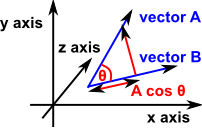
\includegraphics[width=0.4\textwidth]{images/dotProduct.png}
    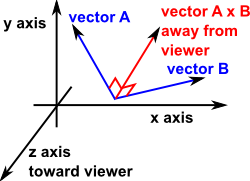
\includegraphics[width=0.4\textwidth]{images/crossProduct.png}
\end{center}


\section{Solid Rotations}

部分内容参考Euclidenan Space网站\cite{Euclideanspace}。

\subsection{Axis Angle}

任意3D旋转都可以表示,给一个solid对象,朝向orientation1,再给另一个朝向orientation2,可以总是
找到一轴axis和一角度angle从orientation1旋转到orientation2.

这个方法是好理解,但是把多个序列的旋转的结果就不好表示了,就需要使用matrix或quaternion啦

\subsection{Euler Angles}
把任意3D旋转分解decompose为三个不同的角度,直觉上会认为这种方式很方便,可是计算上会出现问题,如死锁


当合并旋转时,只有明确旋转顺序order才能确定Euler Angle的姿态。
\begin{description}
    \item [Tait-Bryan angles] \textsf{正序xyz, yzx, zxy; 反序zyx, xzy, yxz。在SLAM(simultaneous localization and mapping)同步定位与建图中应用}
    \item [Proper Euler angles] \textsf{xyx, xzx, yxy, yzy, zxz, zyz,}
\end{description}

旋转的参考,分内旋与外旋。假设世界坐标系XYZ与物体坐标系xyz重合,定义旋转顺序zyx,
旋转角度分别为$\theta, \phi, \psi$。先绕z轴旋转$\theta$后,物体的xy轴发生变化了,z轴不变。
现在旋转第二个旋转角y轴的$\phi$,此时需要内旋与外旋的概念来区分:内旋就是按照物体的坐标系的y轴来旋转,
外旋就是按照世界坐标系的Y轴来旋转。
旋转完成后,第三个旋转角也是如此。

这样一来,Euler Angle的旋转就的必要条件就是有:旋转角度,旋转顺序,旋转方式(内旋还是外旋)。

\begin{center}
    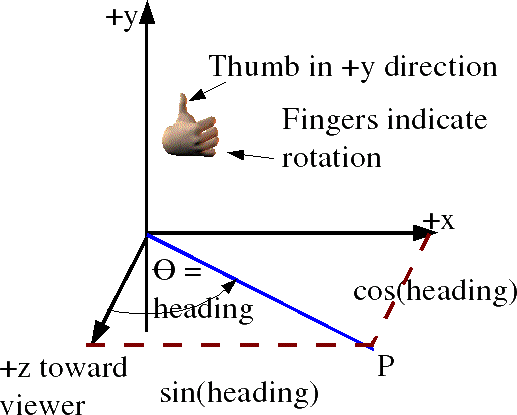
\includegraphics[width=0.3\textwidth]{images/heading.png}
    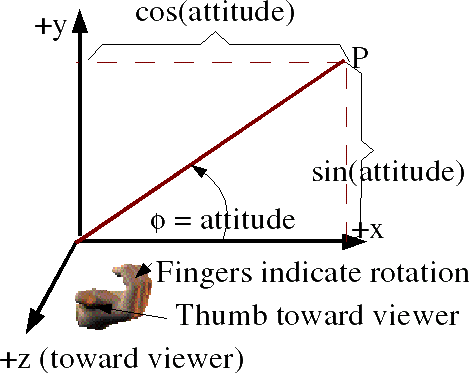
\includegraphics[width=0.3\textwidth]{images/attitude.png}
    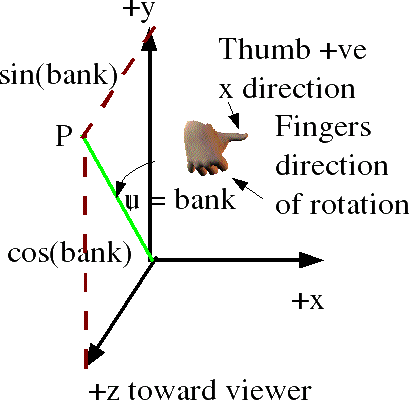
\includegraphics[width=0.3\textwidth]{images/bank.png}
\end{center}

\begin{tabular}{|c|c|c|c|c|c|}
    \hline
  & airplane & telescope & symbol & \hbox{angular velocity} & axis \\ \hline
 \hbox{applied first} & heading & azimuth & \hbox{$\theta$(theta)} & \hbox{yaw偏航} & X \\ \hline
 \hbox{applied second} & attitude & elevation & \hbox{$\phi$(phi)} & \hbox{pitch俯仰} & Z \\ \hline
 \hbox{applied last} & bank & tilt & \hbox{$\psi$(psi)} & \hbox{roll横滚} \\ \hline
\end{tabular}
 
 欧拉角的是为了方便主观去理解,与Axis Angle类型,以理解为主要入手处。

 
 \section{Linear-Transform}

线性变换主要包括缩放、旋转、反射等,不包含平移。线性变换的数学描述为:

\begin{math}
\begin{aligned}
f(\alpha v)=\alpha v, \\
f(u+v)=f(u)+f(v)
\end{aligned}
\end{math}

反射,就是把一个物体变换成它的镜像的映射,在二维空间中,用一条直线作为“镜子”;在三维空间中,使用平面作为“镜子”。


\section{ Matrix }

矩阵Matrix就是线性变换

\subsection{eigenvector}
特征向量
对于一个给定的线性变换(矩阵M,是向量空间E到自身的一个线性变换,可以旋转、反射、拉伸、压缩或变换的组合),它的特征向量V经过这个线性变换之后,得到新的向量U,VU向量共线,但长度可能不一致。
VU的长度缩放的比例称为特征值eigenvalue。

\subsection{minor}
余子式
在n阶行列式D中划去任意选定的k行、k列后,余下的元素按照原来的顺序组成的n-k阶行列式M,M称为
行列式D的k阶子式A的余子式Minor。如果k阶子式A在行列式D中的行和列的标号分别为
$i_{1},i_{2},...,i_{k}$和$j_{1},j_{2},...,j_{k}$。则在A的余子式M前面加一个符号:
\begin{math}
    \begin{aligned}
        {-1}^{(i_{1}+i_{2}+...+i_{k}) + (j_{1}+j_{2}+...+j_{k})}
    \end{aligned}
\end{math}
得到的n-k阶行列式,称为行列式D的k阶子式A的代数余子式Cofactor。

\subsection{determinant}
行列式
行列式其实是一个函数,一个将方阵转换成一个标量的函数。行列式可以看做是有向面积的概念在一般的欧几里得空间中的推广。
行列式表示的是线性变换前后的面积(二维)、(三维为体积)等变化的系数。

n阶行列式det(D)等于其任意行(列)的元素与对应的代数余子式的乘积之和。通过D的i行row来计算

\begin{math}
    \begin{aligned}
   \det(D)=d_{i1}A_{i1}+...+d_{in}A_{in}=\sum_{j=1}^{n}{a_{ij}(-1)^{(i+j)}A_{ij}}
    \end{aligned}
\end{math}

又称为拉普拉斯展开式Laplace expansion,或代数余子式展开式Cofactor expansion
矩阵和行列式是两个完全不一样的概念,行列式的行和列必须相等。

\subsection{adjoint matrix}
伴随矩阵
行列式D的每个元素的代数余子式$A_{ij}$所构成的矩阵,称为矩阵D的伴随矩阵。

\begin{math}
    \begin{aligned}
A^{*}= \begin{pmatrix} A_{11}&A_{21}&A_{...}&A_{n1} \\
A_{12}&A_{22}&A_{...}&A_{n2} \\
A_{...}&A_{...}&A_{...}&A_{...} \\
A_{1n}&A_{2n}&A_{...}&A_{nn} \end{pmatrix} = (A_{ij})^T
\end{aligned}
\end{math}

伴随矩阵就是线性变换的逆操作,再进行一个缩放的结果,缩放的大小与矩阵的行列式的值有关。
伴随矩阵定理:
A是n阶方阵,$A^*$是A的伴随矩阵,则有$AA^*=A^*A=AE$。

\subsection{inverse matrix}
逆矩阵
n阶方阵A,存在n阶方阵B,满足$AB=BA=E$,称方阵A可逆,称方阵B是A的逆矩阵,记为$B=A^{-1}$

由伴随矩阵定理与逆矩阵可得

\begin{math}
    \begin{aligned}
\begin{cases} A^*A=E\\ AA*=|A|E \end{cases} \Rightarrow A^{-1}=\frac{A^*}{|A|}
\end{aligned}
\end{math}


\subsection{正交矩阵}
两个向量的内积为零,就说这两个向量是正交的,在三维空间中,正交的两个向量相互垂直。如果相互正交
向量的长度均为1,又叫做标准正交基。
在矩阵论中,\textbf{实数}正交矩阵是方块矩阵Q,它的转置矩阵是它的逆矩阵,$Q^TQ=QQ^T=I$。
注意实数二字,正交矩阵中的元素都是实数,包含复数并且同样满足正交性质的矩阵是酉矩阵,也就是推广
到复数域之后的“正交矩阵”。

\subsection{相似矩阵}
两个n阶方阵矩阵A与B为相似矩阵当且仅当存在一个n阶方阵的可逆矩阵P,使得$P^{-1}AP=B$或$AP=PB$,
P被称为矩阵A与B之间的相似变换矩阵。
白话就是,矩阵是线性空间中的线性变换的一个描述,在一个线性空间中,只要我们选定一组基,那么对于
任何一个线性变换,都能够用一个确定的矩阵来加以描述。同样的,对于一个线性变换,只要逆选定一组基,
那么就可以找到一个矩阵来描述这个线性变换。换一组基,就得到一个不同的矩阵。所有这些矩阵都是这
同一个线性变换的描述,但又都不是线性变换本身。所有这些同一个线性变换的描述的矩阵互为\textbf{相似矩阵}。

\subsection{过渡矩阵}
transition matrix过渡矩阵这个词在数学语境中有很多地方用得,在线性代数中,它用来表示坐标矩阵的变换。
\newline
设V为n维向量空间,有两个基$S=\{v_1,...,v_n\}$和$T=\{w_1,...,w_n\}$,
过渡矩阵$P_{S \leftarrow T}$从T到S的nxn矩阵,它的列项在基S中的形式为:

\begin{math}
    P_{S \rightarrow T} = [[w_1]_S [w_2]_S ... [w_n]_S]
\end{math}

举例说明:设$S=\{ e_1,e_2,e_3\}$为标准基,$T=\{ w_1=\begin{bmatrix} 1\\ 1\\ 0 \end{bmatrix}\quad, w_2=\begin{bmatrix}0\\1\\2\end{bmatrix}\quad 
, w_3=\begin{bmatrix} 1\\1\\1 \end{bmatrix}\quad \}$。

则有\newline
$P_{S \leftarrow T}=\begin{bmatrix} 1&0&1\\1&1&1\\0&2&1\end{bmatrix}$。

根据这个关系,可以表示$w_3=2e_2+e_3$。

具体数值的例子:设$S=\{ v_1=\begin{bmatrix}1\\2\\3\end{bmatrix}\quad, v_2=\begin{bmatrix}-2\\1\\0\end{bmatrix}\quad 
, v_3=\begin{bmatrix} 1\\0\\1 \end{bmatrix}\quad \}$, $T=\{ w_1=\begin{bmatrix} 1\\1\\0\end{bmatrix}\quad, w_2=\begin{bmatrix}0\\1\\2\end{bmatrix}\quad 
, w_3=\begin{bmatrix} 1\\1\\1 \end{bmatrix}\quad \}$。

求得在基S中的$w_1$的坐标值$x_1,x_2,x_3$。
\newline
由线性关系可得

\begin{math}
    x_1v_1+x_2v_2+x_3v_3=w_1
\end{math}

它的增广矩阵为
\begin{math}
    [ { \begin{array}{c:c:c:c} 
        \begin{matrix} v_1&v_2&v_3 \end{matrix} &
        \begin{matrix} w_1 \end{matrix} &
        \begin{matrix} w_2 \end{matrix} &
        \begin{matrix} w_3 \end{matrix} 
    \end{array}} ] = \Bigg [ {\begin{array}{c:c:c:c} 
        \begin{matrix} 1&-2&1\\2&1&0\\3&0&1 \end{matrix} &
        \begin{matrix} 1\\1\\0 \end{matrix} &
        \begin{matrix} 0\\1\\2 \end{matrix} &
        \begin{matrix} 1\\1\\1 \end{matrix} 
    \end{array}}
    \Bigg ]
\end{math}

对增广矩阵化简得到
\begin{math}
    \Bigg [ {\begin{array}{c:c:c:c} 
    \begin{matrix} 1&0&0\\0&1&0\\0&0&1 \end{matrix} &
    \begin{matrix} 1.5\\-2\\-4.5 \end{matrix} &
    \begin{matrix} 0\\1\\2 \end{matrix} &
    \begin{matrix} 1\\-1\\-2 \end{matrix} 
\end{array}}
\Bigg ]
\end{math}

得到的最后三列就是$[w_1]_S, [w_2]_S,[w_3]_S$, 即过渡矩阵为
\begin{math}
    P_{S \leftarrow T} = \begin{bmatrix}
        1.5 & 0 & 1 \\
        -2 & 1 & -1 \\
        -4.5 & 2 & 2
    \end{bmatrix}
\end{math}

过渡矩阵应用在:骨骼算法中,

\chapter{Geometry}

\section{Conception}

\subsection{Euclidean Geometry}
欧几里得几何学,是对空间物体的刻画,是基于某个维度上的内积inner product。对于空间中的点和线,感兴趣的是它们的距离、角度
等属性,可以通过求其内积获得。

不遵从欧几里得公理系统的几何学,叫做非欧几里得几何学non-Euclidean Geometry

拓扑学Topology是研究几何体连续形变中保持不变的性质。连续的变换最后都能变成一样的两个物体,称为同胚Homeomorphism。

形变是柔软的,像流动的液体一样,这就是流形manifold的概念。一个d维的流形是一个其内任意点局部同胚于欧式空间$R^d$的d维空间。
球面就是一个嵌入三维空间中的二维流形,因为可以把球面任意点周围(局部小区域)看作是一个二维欧式空间。
反过来就是将低维欧式空间在更高维空间进行扭曲就构成了一个流形。

\subsection{manifold}

流形,一般指几何对象的总称,包括各种维数的曲线曲面等。流形学把一组在高维空间中的数据在低维空间中重新表示。

对于描述流形上的点需要坐标,而流形本身是没有坐标的,为了表示流形上的点,需要把流形放入外围空间ambient space
中,使用外围空间坐标来表示。如$R^3$中的球面是个2维的曲面,但球面上的点使用外围$R^3$空间中的坐标来表示。
流形学习可粗略概括为给出$R^3$中的表示,在保持球面上的某些几何性质的条件下,找出一组对应的内蕴坐标intrinsic coordinate 
来表示,它显然是一个二维表达,这个过程也叫做参数化parameterization。

\paragraph{intrinsic}
低维表示也叫做内蕴特征

\paragraph{observation}
高维叫做观察维数,也叫自然坐标。




%-----其他
\clearpage
\chapter{附录}
主要引用的文章以下:
\cite{RAPI}
\cite{Renderer}
\cite{FCG4ed} 计算机图形学基础第四版
%-----

%-----参考文档
\bibliographystyle{plain}
\bibliography{renderer.bib}
%-----

\end{document}